\documentclass[preprint,12pt]{elsarticle}

\usepackage{amsmath}
\usepackage{amssymb}
\usepackage{bm}
\usepackage{graphicx}
\usepackage{booktabs}
\usepackage{placeins}
\usepackage{xcolor}
\usepackage{tikz}
\usetikzlibrary{arrows.meta,calc,positioning}
\usepackage{xeCJK}
\setCJKmainfont{SimSun}
\setCJKsansfont{SimHei}
\usepackage[colorlinks]{hyperref}
\hypersetup{hypertexnames=false}

\graphicspath{{../figures/}}
\newcommand{\todo}[1]{\textcolor{red}{【待定：#1】}}
\newcommand{\jump}[1]{\left[\!\left[#1\right]\!\right]}

\journal{（目标期刊待定 —— 中文审阅稿，正式投稿以英文版为准）}

\makeatletter
\def\abstractname{摘\quad 要}
\def\keywordname{关键词}
\makeatother
\renewcommand{\figurename}{图}
\renewcommand{\tablename}{表}
\renewcommand{\refname}{参考文献}

\begin{document}

\begin{frontmatter}

\title{基于解耦两流体混合流框架的\\充水竖井截留气囊释放喷发（geysering）一维模拟\\
{\normalsize （中文审阅稿 —— 与英文版 \texttt{paper/main.tex} 内容对应）}}

\author{薛子健，周领，朱志伟\corref{cor1}}
\cortext[cor1]{通讯作者}

\begin{abstract}
雨水与合流制排水系统中的喷发（geysering）现象，源于截留气囊经竖井释放并将其上方水柱
喷出地面。系统尺度的预测依赖降阶的一维模型，但现有多数混合流公式将气相处理为边界
条件或集总气囊定律，导致决定``平缓排气''与``喷发''之间分野的气囊--水柱耦合动力学
不在计算状态之内。本文将配套方法学论文中建立的一维解耦两流体切割单元有限体积框架
应用于实验室喷发试验的复现。该框架在分层流段将气体质量与气体动量作为守恒变量保留，
将运动的有压--分层前沿作为状态迁移黎曼问题处理，并把竖井表示为旋转至竖直方向的同一套
一维两流体系统，经由带局部损失闭合的结点与水平管道耦合。所有模拟均从试验初始条件
出发、采用同一冻结求解器配置，不预设释放速率、不脚本化喷发高度、不做逐工况拟合。
模型首先针对已发表的充水通风竖井试验进行评估——加压气囊向部分充水的通风塔释放，
选取不喷发分支的宽塔工况与喷发分支的窄塔工况：两个工况的分支判别均正确。不喷发分支
中，计算所得压头平台、末段排气衰减、气水界面爬升速度与最大水面抬升均与量测吻合。
喷发分支中，塔内水柱的喷发前驻位、压头平台、试验每次重复观测到的喷发至井口、界面与
水面爬升速度、以及气囊泄放时的压头骤降均得到复现，气相事件时刻整体偏早约半个无量纲
时间单位。随后将模型作为分支判别器，在同一冻结配置与全同步结点耦合下针对已发表的
水平管--竖管试验评估：模型复现了已发表双参数喷发判据的两个端元——细竖管喷发（含
驱动喷发的气囊压缩压力激增）与全部宽竖管、小气囊构型的平缓排气——并复现了管端压力
峰值的实测分支分化。其在试验参数扫描上的分类误差严格单向：在分支边界附近低估喷发
（水柱被驱入竖管高处但未喷出），且不产生任何假喷发。该保守偏差溯源至单一已识别闭合
——结点口部的体积中性气水交换，其在两分支上的需求相互冲突——以及结点透射与环状
液膜卷吸的一维局限。针对原型背景交汇室竖井试验的算例组将在后续修订中补充完成。
\end{abstract}

\begin{keyword}
喷发（geysering）\sep 截留气囊 \sep 雨水系统 \sep 竖井 \sep 两流体模型 \sep 瞬变混合流
\end{keyword}

\end{frontmatter}

% ======================================================================
\section{引言}
\label{sec:intro}

喷发（geysering）指雨水及合流制排水系统在快速充水过程中，气水混合物经检查井、跌水井
或通风竖井猛烈喷出的现象。现场观测显示混合物可喷至地面以上数十米，掀翻井盖并危及公共
安全。早期基于水柱纯惯性振荡的解释与现场压力记录相矛盾——喷发竖井附近的测压管水头
从未接近地表~\cite{wright2011note}；真正的驱动机制是大型截留气囊经部分或完全充水的
竖井释放~\cite{vasconcelos2011,wright2011note}。Vasconcelos 与 Wright
\cite{vasconcelos2011} 的实验室试验在受控单井装置上确立了这一气囊释放机制，至今仍是
喷发模型的首要基准。其后的试验研究涵盖了水平管截留气囊向竖管的释放~\cite{cong2017}、
较大尺度竖井中的水体位移与喷发~\cite{muller2017}、以原型跌水井为背景的交汇室上方
雨水喷发~\cite{liu2020}、带井盖检查井的喷发~\cite{zhang2022}，以及喷发的抑制措施
~\cite{qian2020}。喷发事件的物理内核——大型气囊在竖直水柱中上升、膨胀直至膨胀突变
为剧烈——也已在多相流文献中以泰勒气泡膨胀问题的形式被单独分离研究
~\cite{zhouprosperetti2019}。

喷发的数值预测横跨两个极端。三维 VOF 模拟可以细致复现单次实验室事件~\cite{chan2018}，
但其计算代价将其局限于单井、短时间窗，无法用于数百竖井、多暴雨情景的系统尺度筛查。
另一极端上，一维瞬变混合流模型速度足以支撑系统尺度模拟，但现有公式对气相的处理多不
完整。Preissmann 窄缝法与双组分压力法跟踪液相的加压过程~\cite{vasconcelos2006}，而
截留空气即使被表示，也多经由集总气囊定律、预设释放速率或边界条件进入。Vasconcelos 与
Wright \cite{vasconcelos2011} 用于解读自家试验的刚性水柱两相模型需要预先给定气囊与
水柱的拓扑结构，因而只适用于该拓扑已知的几何。由于``平缓排气''与``喷发''之间的
选择取决于气囊压缩、气体侵入竖井、以及井口逆向气水交换的耦合动力学，一个具备预测力的
一维模型必须把气相作为计算状态的一部分携带，而非作为预设的强迫项。

配套方法学论文~\cite{xue2026model}建立了一个针对瞬变封闭管道混合流的一维守恒有限体积
框架：分层流段由解耦两流体系统描述，气体质量与气体动量为守恒变量；满管流段采用弹性管
水锤闭合；运动的有压--分层前沿作为状态迁移黎曼问题处理，嵌入守恒的切割单元前沿追踪
更新。在该框架中，气囊压缩、气体输运与界面失稳增长均为可解析气液动力学的产物。方法学
论文在界面波、段塞生成、气囊压力及综合混合流基准上完成了验证，并包含一个示意性的一维
喷发起动测试；但未对喷发试验做定量对比。

本文提供这一应用层面的评估。将~\cite{xue2026model}的框架原样（公式不变）应用于
竖井与水平管道耦合、截留气囊向竖井释放的实验室喷发试验。竖井被离散为旋转至竖直方向的
同一套一维两流体系统，经由带物理动机局部损失的结点闭合与水平管耦合。所有的分支判别
——自由水面是否在上升的气水界面追上它之前到达井口——均从计算状态中自然产生。

评估按针对已发表试验的算例组（campaign）组织，每组提供一类不同的证据。第一组是
Vasconcelos 与 Wright \cite{vasconcelos2011} 的充水通风竖井试验，从中选取跨越两种
观测分支的两个构型：不喷发分支的大塔工况与喷发分支的小塔工况，考察时间分辨的压力与
界面时程。第二组是 Cong、Chan 与 Lee \cite{cong2017} 的水平管--竖管试验，其系统性
参数研究把喷发结局凝练为一个显式的双参数判据；该组把模型作为分支判别器，在高速摄像
系列与覆盖试验参数范围的 63 构型扫描上进行检验。全部计算采用同一冻结求解器配置，
从试验初始条件出发，不预设释放速率、不脚本化喷发高度、不做逐工况参数拟合。第三组针对
Liu、Shao 与 Zhu \cite{liu2020} 原型背景交汇室试验，检验下游边界分支翻转、喷发高度—峰压
关系及 Series C 瞬变质量振荡解析模型；其余试验研究~\cite{muller2017,zhang2022,qian2020,leon2018}作为佐证性引用。

本文余下部分组织如下：第~\ref{sec:model}~节概述解耦两流体框架，并描述喷发构型所用的
竖井分支与结点闭合；第~\ref{sec:tests}~节给出测试算例及与试验的对比；
第~\ref{sec:discussion}~节讨论对比所揭示的能力与局限；第~\ref{sec:conclusions}~节
给出结论。

% ======================================================================
\section{模型框架}
\label{sec:model}

本节按解读喷发计算所需的程度概述配套方法学论文~\cite{xue2026model}的一维框架，然后
描述喷发构型中使用的竖井分支、结点闭合与截留气囊处理。推导、状态迁移黎曼求解器以及
守恒切割单元前沿追踪算法见~\cite{xue2026model}，此处不再重复。

\subsection{解耦两流体混合流公式}
\label{sec:model:framework}

该框架把封闭管道描述为由运动状态前沿分隔的满管（有压）段与分层气液段的并集。分层段由
\cite{xue2026model} 的解耦两流体平衡律控制，
\begin{equation}
\frac{\partial \mathbf{U}}{\partial t}
+\frac{\partial \mathbf{F}}{\partial x}
=\mathbf{S},
\label{eq:system}
\end{equation}
其守恒状态、通量与正则源项向量为
\begin{equation}
\mathbf{U}=
\begin{bmatrix}
A_g\rho_g \\ \rho_g Q_g \\ A_l \\ Q_l
\end{bmatrix},
\qquad
\mathbf{F}=
\begin{bmatrix}
\rho_g Q_g \\[2pt]
\rho_g Q_g^2/A_g+P_g A_g \\[2pt]
Q_l \\[2pt]
Q_l^2/A_l+\tfrac{1}{2}\Lambda_d A_l^2
\end{bmatrix},
\qquad
\mathbf{S}=
\begin{bmatrix}
0 \\[2pt]
P_g\dfrac{\partial A_g}{\partial x}
-A_g\rho_g g\cos\theta\dfrac{\partial h_l}{\partial x}+\mathcal{S}_g \\[2pt]
0 \\[2pt]
\mathcal{S}_d
\end{bmatrix},
\label{eq:vectors}
\end{equation}
其中 $A_g$、$A_l$ 为气、液横截面积，$\rho_g$ 为气体密度，$Q_g$、$Q_l$ 为气、液体积
流量，$P_g$ 为气体压力，$h_l$ 为液深，$\theta$ 为管道倾角；$\mathcal{S}_g$、
$\mathcal{S}_d$ 为包含轴向重力、壁面摩阻与界面剪切的气、液动量正则源项，剪切闭合
采用标准分层流关联式~\cite{issa2003,taitel1976}。气体质量与气体动量为守恒变量，
因而气体输运、气体惯性、气体可压缩性与剪切驱动的界面增长都属于计算状态。液相动量
通量中的恢复系数为
\begin{equation}
\Lambda_d
=\underbrace{\frac{2gH_g}{A_l}}_{\text{气压项}}
+\underbrace{\frac{\rho_l-\rho_g}{\rho_l}\,g\zeta}_{\text{静水--浮力项}}
-\underbrace{\frac{\rho_g(u_g-u_l)^2}{\rho_l A_g}}_{\text{IKH 滑移项}},
\label{eq:lambda}
\end{equation}
它综合了气压项、静水--浮力项与无粘 Kelvin--Helmholtz（IKH）滑移项的贡献；其中
$H_g$ 为气体压头，$u_g$、$u_l$ 为相速度，$\zeta=\cos\theta/[D\sin(\gamma/2)]$ 为
圆管几何因子（$D$ 为管径，$\gamma$ 为液相圆心角）。解耦液相通量雅可比的特征值
\begin{equation}
\lambda^{\pm}=u_l\pm\sqrt{\Lambda_d A_l}
\label{eq:eigen}
\end{equation}
表明：液相子系统在 $\Lambda_d>0$ 时严格双曲，$\Lambda_d=0$ 处到达中性界面失稳
（IKH）阈值；越过阈值后界面波增长并可形成液桥。

满管段中气相不存在，有压分支由二变量系统
\begin{equation}
\frac{\partial A_l}{\partial t}+\frac{\partial Q_l}{\partial x}=0,
\qquad
\frac{\partial Q_l}{\partial t}
+\frac{\partial}{\partial x}\!\left(\frac{Q_l^2}{A_l}+gA_f h_s\right)
=\mathcal{S}_p
\label{eq:pressurized}
\end{equation}
控制，并以弹性管关系闭合：
\begin{equation}
P-P_{\mathrm{ref}}=\rho_l a^2\,\frac{A_l-A_f}{A_f},
\qquad
h_s=\frac{P-P_{\mathrm{ref}}}{\rho_l g},
\label{eq:elastic}
\end{equation}
其中 $a$ 为（数值）压力波速，$A_f$ 为未变形管道截面积，$h_s$ 为测压管水头，
$\mathcal{S}_p$ 为有压分支正则源项；该分支还原水锤极限。在各极限情形下，
式~(\ref{eq:system})--(\ref{eq:elastic}) 的同一面积变量形式还原出水锤、明渠重力流
（$\Lambda_d\to g\cos\theta/B_l$，$B_l$ 为自由水面顶宽）、界面失稳动力学与近满管
混合流平衡~\cite{xue2026model}。

运动的有压--分层前沿是二变量系统~(\ref{eq:pressurized}) 与四变量
系统~(\ref{eq:system}) 之间的内部边界。其局部闭合与守恒前沿追踪更新在
第~\ref{sec:model:rtrp}--\ref{sec:model:fv}~节中概述，使本文的计算无需借助
~\cite{xue2026model} 即可被解读与复现；推导、活动集求解器的构造与格式在标准基准
上的验证见~\cite{xue2026model}。

该公式的两条性质对喷发问题至关重要。其一，由于气体质量按计算区域守恒，截留气囊被识别为
由液封包围的连通气体区域，其压力由等温状态方程 $P_g = m_g R T / V_g$ 按当前囊内气体
质量 $m_g$ 与体积 $V_g$ 直接给出；不施加任何带预设体积历史的多变气囊定律。其二，由于
分层分支携带气体动量，气体侵入竖井以及井口的逆向气水交换均为解析结果而非预设输入。

\subsection{运动前沿的状态迁移黎曼闭合}
\label{sec:model:rtrp}

在以速度 $w_\Gamma=\dot{x}_\Gamma$ 运动的有压--分层前沿 $x=x_\Gamma(t)$ 处，局部
坐标取有压分支在左、分层分支在右；相反情形经反射得到。两分支共有的守恒量只有液相
质量与液相动量，且理想前沿厚度为零、不存储任何液相量。将混合状态液相平衡在收缩到
前沿的控制体上积分，得到运动 Rankine--Hugoniot 条件
\begin{equation}
\begin{gathered}
Q_{p,\Gamma}-Q_{f,\Gamma}
=w_{\Gamma}\left(A_{p,\Gamma}-A_{l,\Gamma}\right),\\[2pt]
\left(\frac{Q_{p,\Gamma}^2}{A_{p,\Gamma}}+gA_f h_{s,\Gamma}\right)
-\left(\frac{Q_{f,\Gamma}^2}{A_{l,\Gamma}}
+\frac{1}{2}\Lambda_{d,\Gamma}A_{l,\Gamma}^2\right)
=w_{\Gamma}\left(Q_{p,\Gamma}-Q_{f,\Gamma}\right),
\end{gathered}
\label{eq:rh}
\end{equation}
其中下标 $p$、$f$ 分别表示前沿处的有压迹值与分层迹值的液相投影，$h_{s,\Gamma}$ 由
弹性闭合~(\ref{eq:elastic}) 给出。有压侧为满管，气体不穿越前沿，运动系气体条件给出
\begin{equation}
u_{g,\Gamma}=w_\Gamma .
\label{eq:gaskin}
\end{equation}
由于水锤波速 $a$ 远大于混合流前沿速度，总有一条有压声学特征线到达前沿，提供相容关系
\begin{equation}
u_{p,\Gamma}-u_{p,L}+\frac{g}{a}\left(h_{s,\Gamma}-h_{s,L}\right)=0,
\label{eq:compat}
\end{equation}
其中 $L$ 为相邻有压状态。式~(\ref{eq:rh})--(\ref{eq:compat}) 不足以确定全部界面
未知量；剩余信息取决于 $w_\Gamma$ 相对分层液相信号速度
$s_\pm=u_{l,R}\pm c_{l,R}$（$c_{l,R}=\sqrt{\Lambda_{d,R}A_R}$）的位置，后者把可容许
前沿速度划分为慢（$w<s_-$）、中（$s_-\le w\le s_+$）、快（$w>s_+$）三个活动集。

由于正确的活动集在 $w_\Gamma$ 求出之前无法预知，而在每个前沿做分支相关的非线性迭代
在瞬变计算中并不稳健，\cite{xue2026model} 的闭合采用定成本的单步构造：把相容关系
~(\ref{eq:compat}) 与质量跳跃代入动量跳跃后，任一候选速度 $w$ 下的闭合归结为
$A_{p,\Gamma}(w)$ 的标量二次方程与标量动量残差 $R(w)$。由相邻状态构造有限面积预估
\begin{equation}
w_0=\frac{A_{p,L}u_{p,L}-A_R u_{l,R}}{A_{p,L}-A_R},
\label{eq:predictor}
\end{equation}
将其投影到各（略收缩的）活动集区间，在每个区间施加一次闭式 Newton 型残差修正，并按
综合了 Rankine--Hugoniot 残差、离活动集距离与正性罚项的准则选取接受候选。前沿处
不施加任何 Bernoulli 型能量关系。选定迹值定义运动系通量对
$\mathbf{G}_{p,\Gamma}=\mathbf{F}_{p,\Gamma}-w_\Gamma\mathbf{U}_{p,\Gamma}$、
$\mathbf{G}_{f,\Gamma}=\mathbf{F}_{f,\Gamma}-w_\Gamma\mathbf{U}_{f,\Gamma}$，
传递给下述切割单元更新。

\subsection{有限体积推进与切割单元前沿追踪}
\label{sec:model:fv}

在远离前沿处，两分支采用同一套显式有限体积推进：MUSCL--TVD 原始变量重构配 minmod
限制器、分支相关 Rusanov 通量（有压分支取标量耗散 $\max(|u_p|+a)$；分层分支取
块对角耗散，气相速度 $|u_g|+c_g$、分层液相速度 $|u_l|+c_\Lambda$，
$c_\Lambda=\sqrt{\max(\Lambda_d A_l,0)+c_{\mathrm{num}}^2}$）、非分裂单元中心源项
与 SSP--RK2 时间积分。时间步长取分支 CFL 限制与前沿运动限制
$\Delta t_\Gamma=\tfrac{1}{2}\min(\Delta x_p,\Delta x_f)/|w_\Gamma^n|$
的最小值，后者保证前沿每步扫过不超过半个单元。

含前沿单元被划分为长度 $\ell_p$、$\ell_f$（$\ell_p+\ell_f=\Delta x$）的有压与分层
子单元。每步开始时把相邻分支状态传入第~\ref{sec:model:rtrp}~节的闭合；前沿按
$x_\Gamma^{n+1}=x_\Gamma^{n}+w_\Gamma\Delta t$ 推进，各子单元由其外侧分支通量与
前沿处运动系界面通量更新。由于两个子单元平衡使用同一 $w_\Gamma$ 与同一界面迹值，
界面通量与扫掠体积贡献对守恒液相分量与气体质量精确相消：前沿不产生也不湮灭液相
与气体。前沿越过单元界面时对受影响单元做守恒重映（事件重映），接受步之后对剩余的
界面失配施加有界的局部残差松弛。每步结束后识别由液封包围的连通气体区域，其压力由
当前囊内质量与体积按等温状态方程求出。

\subsection{竖井分支}
\label{sec:model:riser}

竖井（通风塔、竖管或跌水井筒）被离散为独立的一维有限体积分支，采用与水平管相同的
面积--动量变量，管道倾角取 $\theta=90^{\circ}$ 使重力沿轴向作用。井顶向大气敞开；
井内自由水面以及贯入其下方的气核由气体体积分数轴向剖面 $\alpha_g(z)$ 表示，而非预设的
气泡形状。竖井状态因此区分自由水面高程 $Y_{fs}$（连续液柱顶端）与气水界面高程
$Y_{int}$（穿越水柱上升的气核前端）——这正是竖井试验所报告的两条轨迹。喷发依照
\cite{vasconcelos2011} 的试验定义诊断：$Y_{fs}$ 在 $Y_{int}$ 追上自由水面之前到达
井顶。

\subsection{结点与局部损失闭合}
\label{sec:model:junction}

竖井底部经由结点闭合与水平管耦合，驱动量为当地管道状态与截留气囊压力。结点交换以气囊
状态方程静压头为驱动压头，并保留以下局部损失要素（即第~\ref{sec:tests}~节所有算例
所用的冻结配置）：

\begin{itemize}
\item 管道与井底之间贯通流的结点进出口损失系数 $K_j=0.75$；
\item 结点携气期间附加的搅混损失 $K_{g}=8.0$，表征井口强耗散的逆向``气上水下''交换
（倒瓶咕嘟效应）；
\item 释放阀蝶阀损失 $K_v=2.0$（阀开后阀板仍留在流道内），并以损失系数节流方式表示
有限的手动开启时间 $t_v=0.25$~s；
\item 排气期间井顶反向下水的 Wallis 型逆流限制（CCFL），限制速度尺度取
$0.5\sqrt{gD_t}$，其中 $D_t$ 为竖井直径。
\end{itemize}

另有三个要素支配\emph{受驱区}（即截留气囊对井内水柱持有超压余量
$H_{a0}>Y_{fs,0}$ 且气体已抵达结点时）的井底耦合；此处先行陈述，其物理动机结合
细塔试验在第~\ref{sec:tests:vw2011:caseB}~节给出：（i）井底以管道\emph{管顶}压力
驱动（竖井在管顶开孔，结点被水封时该处比管底测压管水头线低一个管径）；（ii）与
气囊连通的井内气核为\emph{气囊供压}——井口流入的气体质量抬升气核鼻端（与水平管
管顶气穴同构的``填充至体水平''闭合），而非在底部单元受弥散气泡阻力堆积；（iii）
进气通量受 Wallis 逆流淹没尺度约束，$j_g\le C_w^{2}\sqrt{gD_t\,\Delta\rho/\rho_l}$，
$C_w=0.9$。这些闭合只使用几何事实与文献尺度常数；在非受驱区（算例组~1 的 Test~A）
它们不激活，井底沿用管底基准耦合，两种基准处理的合并问题见
第~\ref{sec:discussion}~节。

一旦截留气囊与竖井连通且气体突破液封，排气即行``闩锁''：气囊经竖井持续泄放，不再被
间歇段塞重新封闭。该闩锁反映的试验事实是：贯通之后的释放表现为持续（尽管有振荡）的
排放，而非一系列彼此独立的封闭--突破事件。

\subsection{数值配置}
\label{sec:model:numerics}

第~\ref{sec:tests}~节所有计算采用同一冻结求解器配置：水平向网格间距
$\Delta s=0.02$~m，竖井网格间距 $\Delta z=0.01$~m，CFL 数 0.35，满管分支数值弹性
波速降为 $a=28$~m/s。降波速使满管段在气囊与竖井时间尺度上表现为有效不可压
（重力波尺度为 $\sqrt{gD}\approx 1$~m/s），同时避免网格尺度微空穴处的刚性声学振铃；
本文研究的喷发动力学由气囊压缩与重力波主导，而非水锤主导。气体热力学取等温，
$R=287$~J/(kg\,K)，$T=293$~K；液体密度 $\rho_l=998$~kg/m$^3$。任何损失系数或数值
参数在各算例之间均不作调整；唯一随工况变化的要素是第~\ref{sec:model:junction}~节
按流态触发的井底处理（受驱区取管顶基准、气囊供压、淹没限；否则取管底基准），其切换
依据的是物理状态而非算例身份。

% ======================================================================
\section{测试算例}
\label{sec:tests}

评估按针对已发表喷发试验的算例组序列组织。每组内部选取跨越试验观测分支的构型，全部
构型采用第~\ref{sec:model:numerics}~节的同一冻结求解器配置计算。模拟从文献记载的试验
初始条件出发；竖井运动、气体释放与分支判别均为计算结果。不使用预设释放速率、脚本化
喷发高度、溢流累积器或逐工况参数拟合。

从试验喷发文献中选取三组算例，每组贡献一类不同的证据。第一组
（第~\ref{sec:tests:vw2011}~节）复现 Vasconcelos 与 Wright \cite{vasconcelos2011}
的充水通风竖井试验——被引最多的受控喷发试验、喷发模型的标准基准——在两个分支上
检验时间分辨的时程：Test~A 为不喷发分支，Test~B 为喷发分支。第二组
（第~\ref{sec:tests:cong2017}~节）复现 Cong、Chan 与 Lee \cite{cong2017} 的
水平管/竖管试验，这是唯一把结局凝练为显式双参数喷发判据的试验；因此它检验的是模型
作为分支判别器在系统性参数扫描上的表现，而非个别时程。第三组
（第~\ref{sec:tests:liu2020}~节）针对 Liu、Shao 与 Zhu \cite{liu2020} 的原型背景
交汇室试验，把实验室基准接续到现场尺度的跌水井几何。其余试验研究——现场观测
\cite{wright2011note}、为三维 CFD 标定设计的较大尺度释放 \cite{muller2017}、带井盖
检查井喷发 \cite{zhang2022}、抑制措施研究 \cite{qian2020}、以及竖管剧烈喷发
\cite{leon2018}——作为佐证性引用而非复现对象：或因其几何未受控到可作一维对比的程度，
或因其关注点（井盖动力学、抑制装置、闪蒸驱动喷发）在本文所研究的截留气囊释放机制之外。

\subsection{算例组 1：充水通风竖井（Vasconcelos 与 Wright，2011）}
\label{sec:tests:vw2011}

\cite{vasconcelos2011} 的装置由直径 $D=0.094$~m、两端封闭的水平亚克力管，装于距上游端
$3.516$~m 处联轴节上、长 $L=0.610$~m、直径 $D_t$ 可变的通风塔，以及由蝶阀与充水段
隔开、长 $0.546$~m 的上游气室组成（图~\ref{fig:apparatus}）。气室预先加压至初始表压头
$H_{a0}$，塔内预充水至初始水位 $Y_{fs,0}$，手动开阀（历时小于 1~s）即开始一次试验。
加压气囊随后沿管顶向塔推进，并经塔内水柱排出。压力传感器位于阀下游 $1.07$~m 处。
试验矩阵变化 $D_t\in\{57.1,\,44.4,\,25.4,\,12.7\}$~mm（$D_t/D=0.607$--$0.135$）、
$H_{a0}\in\{0.305,\,0.610,\,0.915\}$~m、$Y_{fs,0}\in\{0.254,\,0.356,\,0.457\}$~m。
控制变量被确认为塔径：$D_t/D=0.607$ 时水面抬升从未超过 $L$ 的 10\%，而
$D_t/D=0.135$ 时每次重复水面均到达塔顶。

\begin{figure}[htbp]
\centering
\begin{tikzpicture}[x=2.6cm, y=2.6cm, line cap=round]
\def\ph{0.10}
\def\towx{3.516}
\def\toww{0.06}
\def\towh{0.61}
\fill[blue!25] (0.546,-\ph) rectangle (4.006,\ph);
\fill[blue!25] (\towx-\toww,\ph) rectangle (\towx+\toww,\ph+0.356);
\fill[gray!15] (0,-\ph) rectangle (0.546,\ph);
\fill[gray!15] (\towx-\toww,\ph+0.356) rectangle (\towx+\toww,\ph+\towh);
\draw[thick] (0,\ph) -- (\towx-\toww,\ph);
\draw[thick] (\towx+\toww,\ph) -- (4.006,\ph);
\draw[thick] (0,-\ph) -- (4.006,-\ph);
\draw[thick] (0,-\ph) -- (0,\ph);
\draw[thick] (4.006,-\ph) -- (4.006,\ph);
\draw[thick] (\towx-\toww,\ph) -- (\towx-\toww,\ph+\towh);
\draw[thick] (\towx+\toww,\ph) -- (\towx+\toww,\ph+\towh);
\node[above] at (\towx,\ph+\towh) {\scriptsize 顶部敞开};
\draw[very thick] (0.546,-\ph-0.03) -- (0.546,\ph+0.03);
\node[above] at (0.546,\ph+0.05) {\scriptsize 蝶阀};
\fill (1.616,-\ph) circle (0.02);
\draw (1.616,-\ph) -- (1.9,-\ph-0.08);
\node[right] at (1.9,-\ph-0.08) {\scriptsize 传感器（阀下游 $1.07$ m）};
\node at (0.27,0) {\scriptsize 气，$H_{a0}$};
\node at (2.3,0) {\scriptsize 水};
\node[left] at (\towx-\toww-0.02,\ph+0.18) {\scriptsize $Y_{fs,0}$};
\draw[{Latex}-{Latex}] (\towx-\toww-0.09,\ph) -- (\towx-\toww-0.09,\ph+0.356);
\node[right] at (\towx+\toww+0.02,\ph+0.30) {\scriptsize $L=0.610$ m，直径 $D_t$};
\draw[{Latex}-{Latex}] (0,-\ph-0.16) -- (0.546,-\ph-0.16)
  node[midway,below] {\scriptsize $0.546$ m};
\draw[{Latex}-{Latex}] (0.546,-\ph-0.26) -- (3.516,-\ph-0.26)
  node[midway,below] {\scriptsize $2.970$ m};
\draw[{Latex}-{Latex}] (3.516,-\ph-0.16) -- (4.006,-\ph-0.16)
  node[midway,below] {\scriptsize $0.490$ m};
\node[right] at (4.02,0) {\scriptsize 封闭};
\node[left] at (-0.02,0) {\scriptsize 封闭};
\end{tikzpicture}
\caption{按模型离散方式绘制的 Vasconcelos 与 Wright \cite{vasconcelos2011} 装置示意
（横向不按比例）。水平管（$D=0.094$~m）两端封闭；上游气室容纳加压气囊；通风塔
（长 $L=0.610$~m，直径 $D_t$）顶部敞开，预充水至 $Y_{fs,0}$。}
\label{fig:apparatus}
\end{figure}

选取跨越两种分支的两个构型（表~\ref{tab:cases}）。依照 \cite{vasconcelos2011}，
结果以塔长与塔重力速度尺度无量纲化：高程与压头为 $Y^{*}=Y/L$、$H^{*}=H/L$，时间为
$T^{*}=t\sqrt{gD_t}/L$。喷发定义为自由水面 $Y^{*}_{fs}$ 在上升的气水界面
$Y^{*}_{int}$ 追上它之前到达塔顶（$Y^{*}=1$）。

\begin{table}[htbp]
\centering
\caption{从 \cite{vasconcelos2011} 试验矩阵中选取的工况。}
\label{tab:cases}
\begin{tabular}{lcccccc}
\toprule
工况 & $D_t$ (mm) & $D_t/D$ & $H_{a0}$ (m) & $Y_{fs,0}$ (m) &
$L/\sqrt{gD_t}$ (s) & 观测分支 \\
\midrule
A & 57.1 & 0.607 & 0.305 & 0.356 & 0.815 & 不喷发 \\
B & 12.7 & 0.135 & 0.610 & 0.356 & 1.728 & 喷发（每次重复） \\
\bottomrule
\end{tabular}
\end{table}

模型几何严格按照装置设置：上游气室 $0.546$~m（即初始气囊体积
$3.79\times10^{-3}$~m$^3$），中段管 $2.970$~m，下游封闭管 $0.490$~m，塔位于
$x=3.516$~m，传感器采样点位于 $x=1.616$~m。初始气囊压力
$P_{a0}=P_{\mathrm{atm}}+\rho_l g H_{a0}$；阀下游管道与塔内 $Y_{fs,0}$ 以下初始为
静止充水。对比用试验曲线由 \cite{vasconcelos2011} 已发表图件数字化获得（压头取自其
图~5 与图~6；水面与界面轨迹取自其图~7 与图~8，各 3 次试验重复）；数字化的各次重复
以散点或包络带形式展示。

\subsubsection{Test A：大塔，不喷发分支（$D_t/D=0.607$）}
\label{sec:tests:vw2011:caseA}

试验中该构型的气囊平缓排出、不发生喷发：塔内水面抬升小于 $L$ 的 10\%，传感器压头在
气囊泄放期间维持 $H^{*}\approx0.54$ 的长平台，气囊排空后压头衰减归零。计算复现了该
分支：水面最高 $Y^{*}_{fs}=0.66$（实测最大 0.63），上升气核在塔内追上自由水面，
不发生溢流。

图~\ref{fig:caseA_pressure} 对比了传感器压头。模型在完整泄放窗口
$1\lesssim T^{*}\lesssim7.5$ 内复现平台水平（周期平均 $H^{*}=0.51$，实验数字化平台
$H^{*}=0.54$），并复现与气囊排空相伴的末段衰减：模型自 $T^{*}\approx8.9$ 起跌，
实验为 $8.3$。可见两点差异。其一，$0<T^{*}\lesssim5$ 内模型原始迹线携带周期约
$0.7$~s、于 $t\approx4$~s 内衰减的水柱--气囊弹簧振荡；质量守恒与相位核查确认其为
释放活塞的真实体积--压力振荡而非数值伪振，但实验迹线阻尼更强。图中模型曲线因此以
$0.8$~s 窗口做周期平均。其二，模型的排气阶段偏晚且更缓：实测压头自 $T^{*}\approx8.3$
起跌、约 $9.3$ 归零，而模型平台保持至 $T^{*}\approx8.9$、至窗口末端降至约
$H^{*}\approx0.21$。两者同源于耗散气穴波速下气囊经塔泄放的喂给速率降低——
到达时刻的对齐收益与排气阶段的滞后互为代价（见第~\ref{sec:discussion}~节）。

\begin{figure}[htbp]
\centering
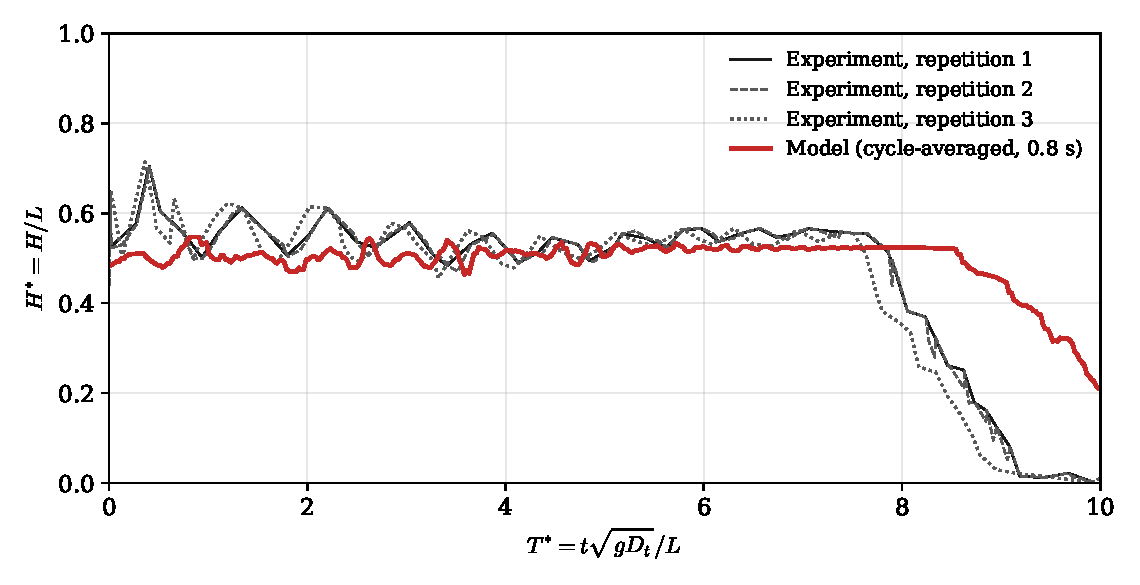
\includegraphics[width=\textwidth]{caseA_pressure.pdf}
\caption{Test A（$D_t/D=0.607$，$H_{a0}=0.305$~m，$Y_{fs,0}=0.356$~m）：传感器压头
$H^{*}$ 随 $T^{*}$ 变化。黑色线：\cite{vasconcelos2011} 图~5 的三次试验重复
（逐点手工数字化）；红线：模型（$0.8$~s 窗口周期平均）。}
\label{fig:caseA_pressure}
\end{figure}

图~\ref{fig:caseA_levels} 在文献发表的观测窗口（$T^{*}=7$--$10$，
\cite{vasconcelos2011} 图~7）内对比塔内自由水面与气水界面轨迹。模型在整个
泄放平台期将水面保持在 $Y^{*}_{fs}\approx0.6$ 附近，与实测水平一致；界面穿塔爬升的
斜率正确：拟合无量纲界面速度 $V^{*}_{int}=0.41$，实验 Table~2 平均值 $0.39$，该塔径
照片估算值 $0.50$。模型界面在 $T^{*}=7.5$ 离开塔底，落在三次试验重复起爬时刻
（$7.3$、$7.8$、$7.9$）的散布之内；在 $T^{*}=8.8$ 追上水面（实验 $8.4$）
（表~\ref{tab:caseA_metrics}）。水位时程有两点系统性差异。其一，实测水面在界面爬升
期间缓升（$0.59$ 升至 $0.65$），\cite{vasconcelos2011} 将其归因于降压气囊进塔后的
膨胀；模型水位停在平台值，因为井口体积中性的逆向交换让气体穿过静立水柱而无净体积
注入，爬升期水面速度 $V^{*}_{fs}\approx0$（实测 $0.048$；最大水位本身吻合：模型
$0.66$ 对实测 $0.63$）。其二，界面到达水面后，实测塔内水位维持约 $0.6L$ 至观测窗
结束，而模型在排气建立后水位下降偏快；井口逆流限制
（第~\ref{sec:model:junction}~节）约束了但未消除这一偏快的下泄。两点差异同源于
第~\ref{sec:discussion}~节讨论的液膜连通气囊拓扑。

\begin{figure}[htbp]
\centering
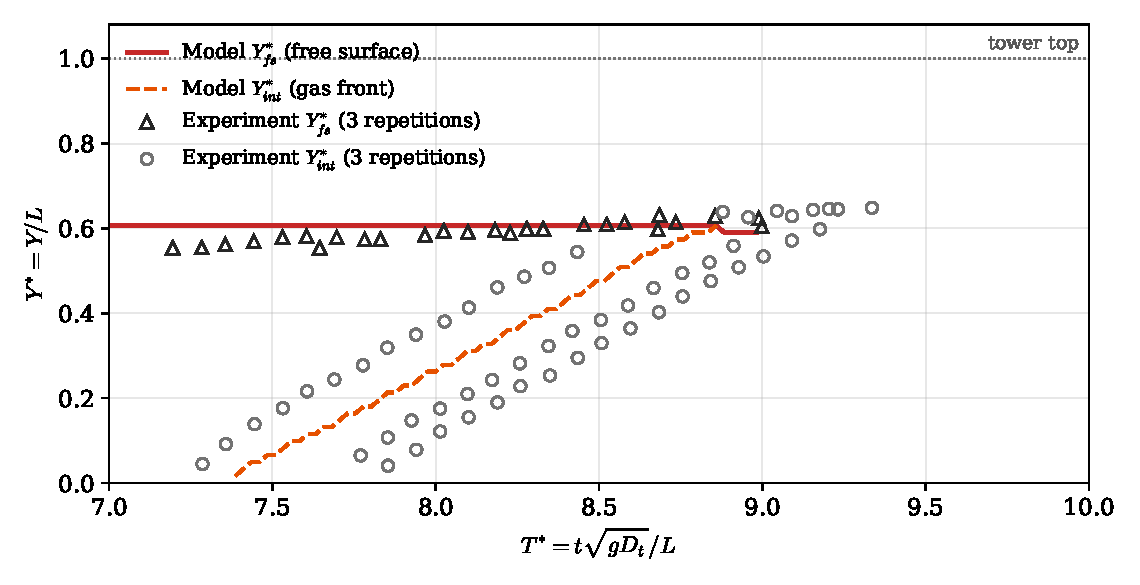
\includegraphics[width=\textwidth]{caseA_levels.pdf}
\caption{Test A：文献发表观测窗口（$T^{*}=7$--$10$）内塔内自由水面高程
$Y^{*}_{fs}$（实线）与气水界面高程 $Y^{*}_{int}$（虚线）随 $T^{*}$ 变化。
散点为 \cite{vasconcelos2011} 图~7 数字化的三次试验重复
（三角：水面；圆圈：界面）。模型气相前沿曲线画至其追上自由水面的时刻为止
（此后两界面合并，不再存在独立前沿）；模型水面曲线画至实验数据覆盖范围为止。
浅色曲线为刚体平移 $+0.75$ 个时间单位的模型气相前沿——该值为模型离底时刻相对
三次重复平均起爬时刻的偏移，平移后计算爬升落于三次重复的散布之内
（三次重复起爬时刻本身散布 $0.6$ 个时间单位）。}
\label{fig:caseA_levels}
\end{figure}

图~\ref{fig:caseA_snapshots} 将 \cite{vasconcelos2011} 图~4 的摄影序列与界面爬升期间
按相同 $0.14$~s 间隔输出的塔内计算快照并列。计算行中的气核宽度直接取当地两流体气体分数，
不做阈值化。计算的前沿位置在整个序列中与摄影前沿的偏差在 $0.03$~m 以内；摄影区间内
的平均前沿速度试验估算为 $0.375$~m/s，模型拟合窗口内为 $0.31$~m/s。

\begin{figure}[htbp]
\centering
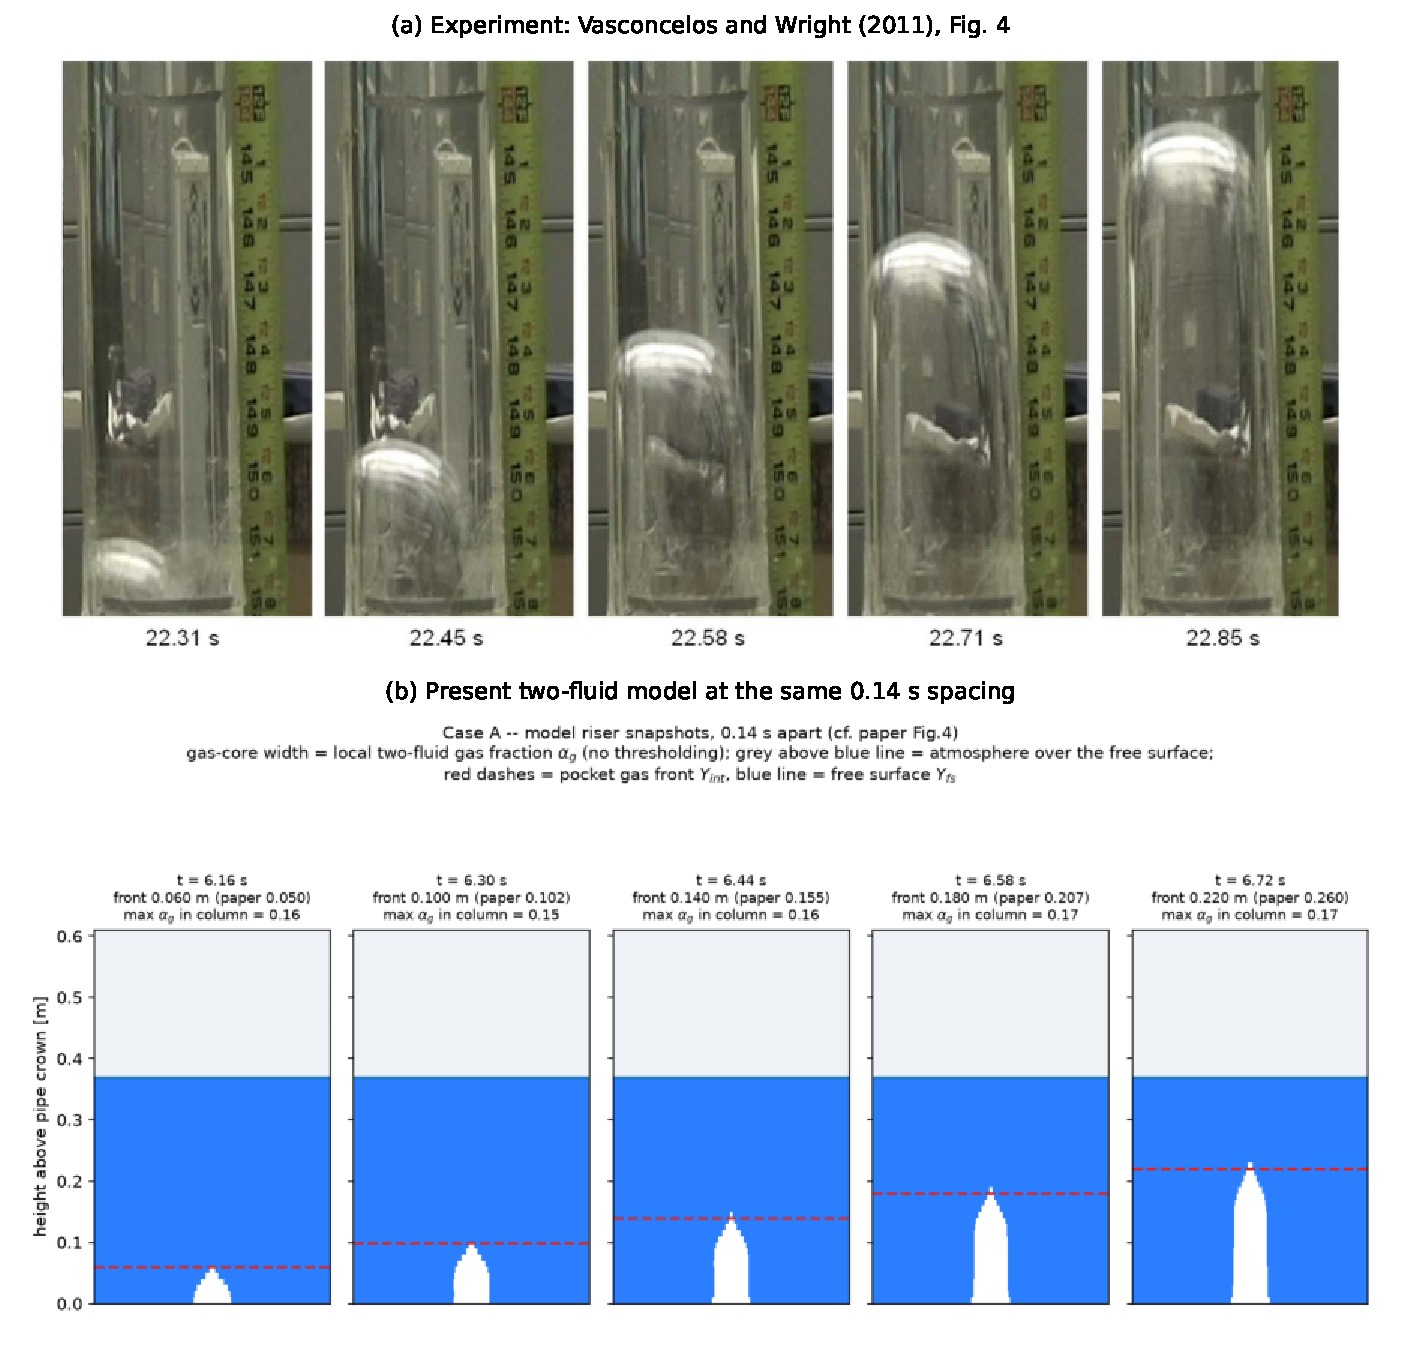
\includegraphics[width=\textwidth]{caseA_fig4_experiment_model.pdf}
\caption{Test A 与 \cite{vasconcelos2011} 图~4 的直接对照。上：论文发表的五帧试验
照片；下：相同 $0.14$~s 间隔的计算塔内相分布。蓝：水；白：气核（当地两流体气体
分数）；灰：自由水面上方大气。红色虚线为计算的气囊前沿 $Y_{int}$；各栏标题给出计算
与摄影的前沿高程。}
\label{fig:caseA_snapshots}
\end{figure}

\begin{table}[htbp]
\centering
\caption{Test A：实测与计算对照。时间为无量纲（$T^{*}=t\sqrt{gD_t}/L$）；速度以
$\sqrt{gD_t}$ 归一化。实验值数字化自 \cite{vasconcelos2011}（图~4、5、7 与
Table~2）。}
\label{tab:caseA_metrics}
\resizebox{\textwidth}{!}{%
\begin{tabular}{lcc}
\toprule
指标 & 实验 & 模型 \\
\midrule
分支 & 不喷发 & 不喷发 \\
最大水面抬升 $Y^{*}_{fs,\max}$ & 0.63 & 0.67 \\
压头平台 $H^{*}$ & 0.54 & 0.52 \\
末段压头衰减起始 $T^{*}$ & 8.3 & 7.8 \\
界面离开塔底 $T^{*}$ & 7.3 & 6.9 \\
界面追上自由水面 $T^{*}$ & 8.4 & 8.1 \\
界面爬升速度 $V^{*}_{int}$ & 0.39（Table~2），0.50（图~4） & 0.42 \\
爬升期水面速度 $V^{*}_{fs}$ & 0.048 & $\approx0$ \\
\bottomrule
\end{tabular}%
}
\end{table}

为避免只展示 \cite{vasconcelos2011} 图~10 中的界面轨迹与压头两个面板，
图~\ref{fig:caseA_tpa_full} 进一步给出该相邻工况
（$D_t/D=0.607$、$H_{a0}=0.305$~m、$Y_{fs,0}=0.254$~m）的完整五联图。
计算的界面速度在连贯爬升期与试验及原 TPA 模型处于相近水平；但计算水面速度缺少实测
的振荡性正脉冲，这与水面轨迹中已经看到的塔口体积中性交换局限相一致。

\begin{figure}[htbp]
\centering
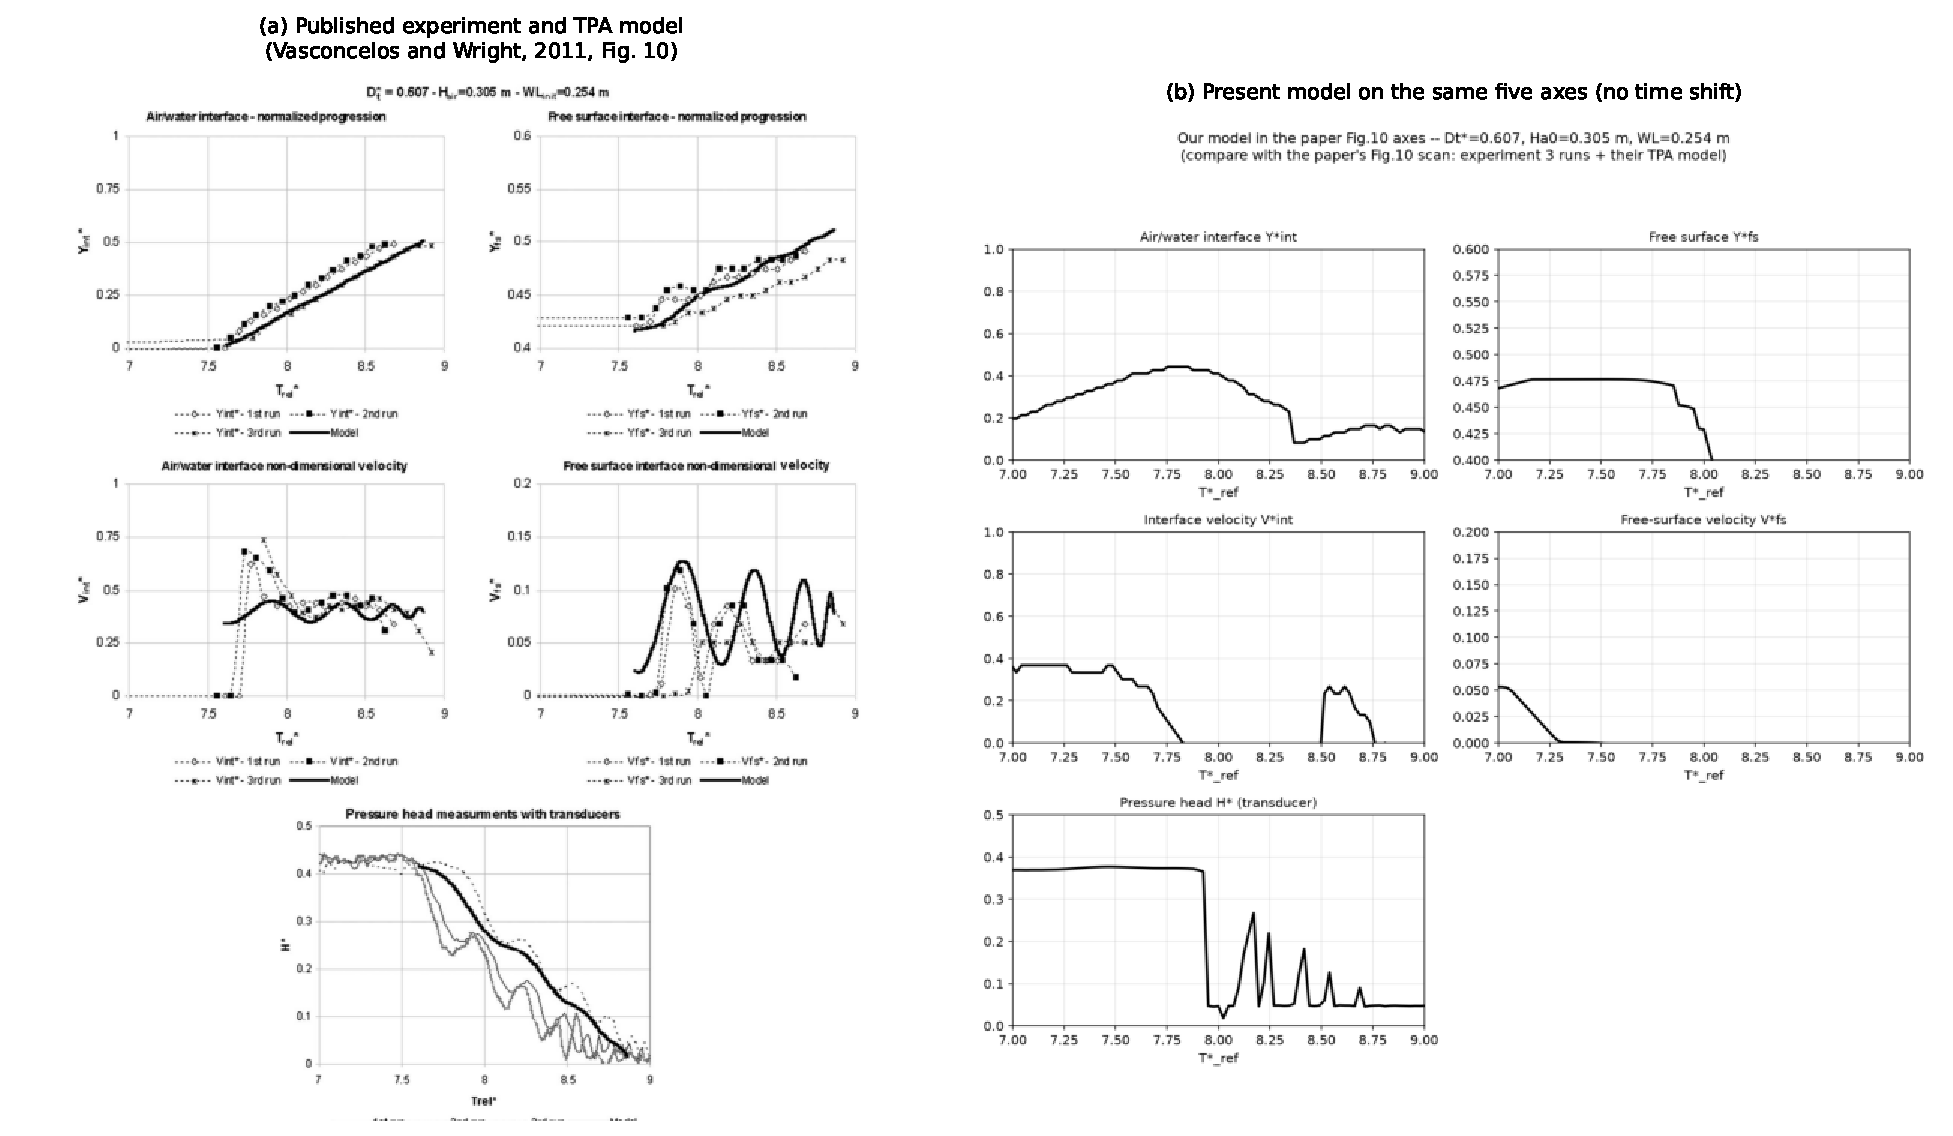
\includegraphics[width=\textwidth]{caseA_fig10_full_comparison.pdf}
\caption{Campaign 1，相邻 $Y_{fs,0}=0.254$~m 工况：对应
\cite{vasconcelos2011} 图~10 的完整五联对照。左：发表的三次试验与 TPA 模型；
右：本模型在同一坐标轴上的结果，不施加时间平移。五个面板依次为
$Y^{*}_{int}$、$Y^{*}_{fs}$、$V^{*}_{int}$、$V^{*}_{fs}$ 与 $H^{*}$。
左侧源图在此保留用于直接视觉核验。}
\label{fig:caseA_tpa_full}
\end{figure}

\FloatBarrier

\subsubsection{Test B：小塔，喷发分支（$D_t/D=0.135$）}
\label{sec:tests:vw2011:caseB}

试验中该构型每次重复均喷发：气囊沿管顶推进期间，塔内水位先抬升至
$Y^{*}_{fs}\approx0.82$ 的准静态驻位；气水界面于 $T^{*}\approx3.65$ 进塔后，含气的
自由水面加速上升、于 $T^{*}\approx3.9$ 到达塔顶，早于界面（约 $T^{*}\approx4.1$
到顶）追上它。传感器压头维持 $H^{*}\approx0.76$ 的平台，并在气囊泄放的
$T^{*}\approx4.05$ 处陡然塌落。

结点闭合中有三个要素为此细塔工况专设，先于对比陈述；每一要素都基于几何事实或
文献尺度常数，而非拟合值。（i）\emph{管顶基准的塔基耦合}：通风塔在管道\emph{管顶}
开孔，故塔基压力应取管顶压力——结点被水封时它比管底测压管水头线低一个管径——
而非管底值；若用管底耦合，细塔会被多至 $\rho_l g D$（$0.15L$）的虚假驱动压头
过度驱动，其水柱自释放瞬态起即被钉在井口。（ii）\emph{气囊供压的连通气核}：
气囊持有超压且结点携气期间，塔内自底部连通的气体与气囊构成一体，井口流入的气体质量
抬升气核\emph{鼻端}（与水平管中管顶气穴所用的``填充至体水平''闭合同构），而非堆积在
底部单元——在那里弥散气泡阻力会把爬升限制在泰勒尺度。（iii）\emph{淹没限进气}：
细塔的受驱吹通受逆流淹没（Wallis）尺度约束，表观气速
$j_g\le C_w^{2}\sqrt{gD_t\,\Delta\rho/\rho_l}$，光滑管口取 $C_w=0.9$。实测爬升速度
$V^{*}_{int}=1.43$（\cite{vasconcelos2011} Table~2）正是气囊供压气核的淹没限鼻端
速度；没有任何系数向它调校。要素（ii）（iii）在 Test~A 中不激活（该工况气囊无超压
余量，$H_{a0}<Y_{fs,0}$）；Test~A 沿用管底基准耦合，两种塔基基准处理合并为单一
结点闭合的问题在第~\ref{sec:discussion}~节讨论。

采用上述闭合后，计算在一个整体时间偏移之内定量复现了喷发分支
（图~\ref{fig:caseB_pressure} 与~\ref{fig:caseB_levels}，
表~\ref{tab:caseB_metrics}）。自由水面抬升至准静态驻位 $Y^{*}_{fs}=0.84$
（实测 $0.82$）——即等温气囊膨胀与塔内水柱相平衡的水位——并保持至界面进塔；
喷发随后进行至井口，与试验每次重复一致。以管顶基准（传感器测点与塔基高程）读取的
传感器平台为 $H^{*}=0.76$，与实测 $0.76$ 一致；管底基准的原始记录（$0.91$）以浅色
迹线保留于图~\ref{fig:caseB_pressure}，且实测平台与``等温气囊状态 + 实测塔水位 +
管顶基准''的静力学组合自洽至 $0.02L$ 以内。爬升运动学跟随实测：拟合界面速度
$V^{*}_{int}=1.19$（Table~2 平均 $1.43$；偏低，但远高于弥散阻力闭合给出的泰勒尺度
$0.35$），喷发前最后爬升段的水面速度
$V^{*}_{fs}=0.42$（实测 $0.44$）。气囊泄放时压头的``平台--骤降''形态以实测形状复现。

剩余偏差是气相事件序列的系统性时间偏移：界面进塔 $T^{*}=3.15$（实测 $3.65$）、
水面到顶 $3.32$（实测 $3.90$）、界面到 $0.85L$ 为 $3.54$（实测 $3.85$）、压头骤降
$3.73$（实测 $4.05$）——一致偏早 $0.3$--$0.6$ 个时间单位，与 Test~A 偏早方向相同、
量级相当。由于四个事件几乎按同一常量偏移，序列结构（进塔 $\rightarrow$ 喷发
$\rightarrow$ 贯通 $\rightarrow$ 骤降）与事件间隔均正确；偏移源于塔上游的释放阶段
（手动阀开启表示与管顶气穴沿水平管的输运），而非竖井动力学本身。
图~\ref{fig:caseB_levels} 因此同时
给出刚体平移 $+0.54$ 个时间单位的模型轨迹，其与实测爬升在三次重复的散布范围内重合。
模型早期迹线还携带 Test~A 中提到的欠阻尼释放活塞振荡（实验迹线约一个时间单位内
衰减；\cite{vasconcelos2011} 的装置示意图对这一释放振荡有明确标注），释放摆动期间
模型水柱曾短暂溅至井口，随后回落至准静态驻位。

\begin{figure}[htbp]
\centering
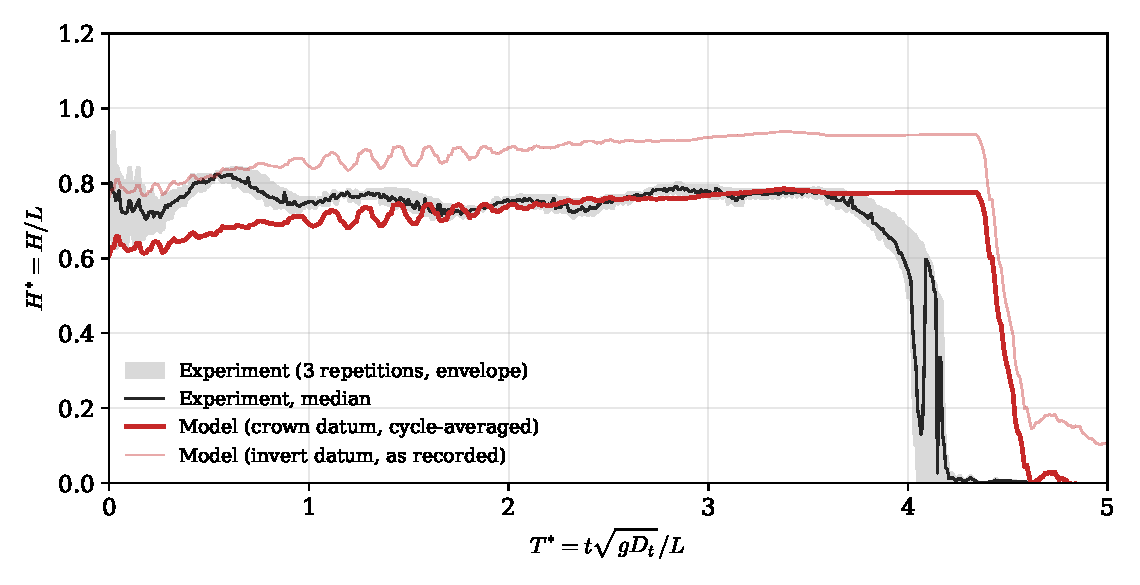
\includegraphics[width=\textwidth]{caseB_pressure.pdf}
\caption{Test B（$D_t/D=0.135$，$H_{a0}=0.610$~m，$Y_{fs,0}=0.356$~m）：传感器压头
$H^{*}$ 随 $T^{*}$ 变化。灰色带与深色线：\cite{vasconcelos2011} 图~6 三次试验重复的
数字化包络与中位线；红色粗线：模型压头（$0.4$~s 窗口周期平均，管顶基准，即传感器
测点与塔基高程，相对管底记录 $-D/L$）；红色浅线：同一迹线的管底基准原始记录。}
\label{fig:caseB_pressure}
\end{figure}

\begin{figure}[htbp]
\centering
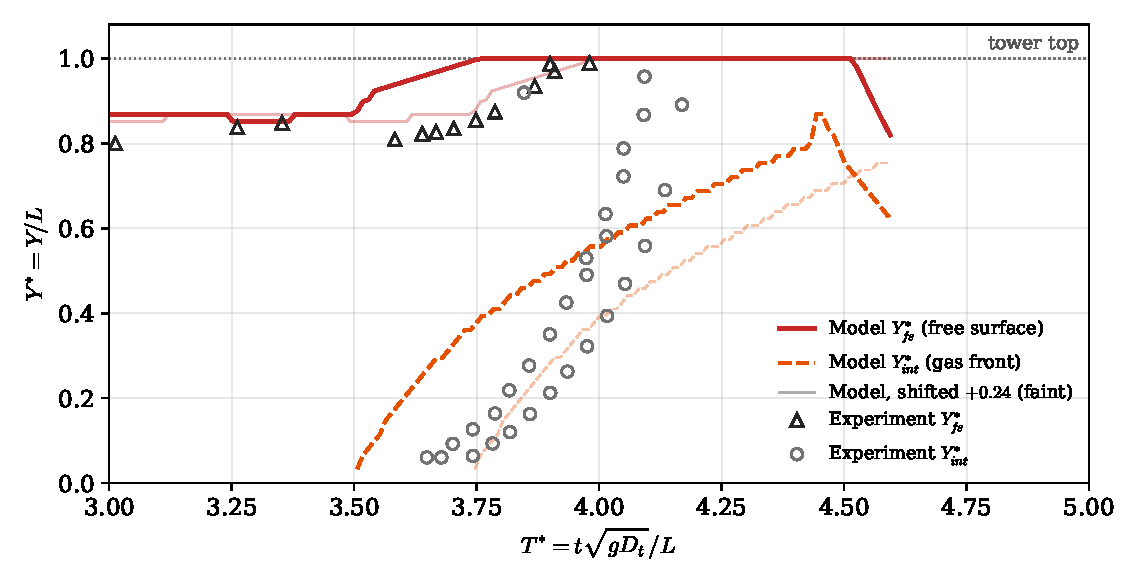
\includegraphics[width=\textwidth]{caseB_levels.pdf}
\caption{Test B：发表观测窗口（$T^{*}=3$--$5$）内塔内自由水面高程 $Y^{*}_{fs}$
（实线）与气水界面高程 $Y^{*}_{int}$（虚线）随 $T^{*}$ 变化。散点为
\cite{vasconcelos2011} 图~8 数字化试验重复（三角：水面；圆圈：界面）。浅色曲线为
刚体平移 $+0.54$ 个时间单位的模型轨迹，用以把爬升运动学与管顶气穴系统性提前抵塔的
影响分离；模型曲线画至实验数据覆盖范围为止。}
\label{fig:caseB_levels}
\end{figure}

\begin{table}[htbp]
\centering
\caption{Test B：实测与计算对照。时间为无量纲（$T^{*}=t\sqrt{gD_t}/L$）；速度以
$\sqrt{gD_t}$ 归一化。实验值数字化自 \cite{vasconcelos2011}（图~6、图~8 与
Table~2）。模型压头平台按管顶基准读取（管底记录为 $0.92$）。}
\label{tab:caseB_metrics}
\begin{tabular}{lcc}
\toprule
指标 & 实验 & 模型 \\
\midrule
分支 & 喷发（每次重复） & 喷发 \\
喷发前水面驻位 $Y^{*}_{fs}$ & 0.82 & 0.84 \\
压头平台 $H^{*}$（管顶基准） & 0.76 & 0.76 \\
界面爬升速度 $V^{*}_{int}$ & 1.43 & 1.19 \\
水面爬升速度 $V^{*}_{fs}$ & 0.44 & 0.42 \\
界面进塔 $T^{*}$ & 3.65 & 3.15 \\
自由水面到达塔顶 $T^{*}$ & 3.90 & 3.32 \\
界面到达 $0.85L$ $T^{*}$ & 3.85 & 3.54 \\
气囊泄放压头骤降 $T^{*}$ & 4.05 & 3.73 \\
\bottomrule
\end{tabular}
\end{table}

综合来看，Tests A 与 B 表明该框架能从第一性出发判别 \cite{vasconcelos2011} 的两种
试验分支——宽塔平缓排气不溢流、细塔喷发至井口——并在两个分支上复现压力平台、
细塔水柱的喷发前驻位与喷发过程、末段泄放衰减起始与界面运动学。剩余偏差为气相事件
一致的提前（Test~A 为 $0.3$--$0.4$、Test~B 为 $0.3$--$0.6$ 个时间单位，与手动开阀
时间的不确定度同量级）与欠阻尼的释放振荡；为 Test~B 引入的细塔闭合要素及其与宽塔
配置的合并问题见第~\ref{sec:discussion}~节。

\FloatBarrier

\subsection{算例组 2：水平管截留气囊向竖管释放（Cong、Chan 与 Lee，2017）}
\label{sec:tests:cong2017}

\subsubsection{试验装置与工况}
\label{sec:tests:cong2017:setup}

\cite{cong2017} 的装置由直径 $D=0.05$~m、长约 $6$~m 的水平亚克力管组成，上游接
定水头水箱，管上经 T 型结点装有高 $1.8$~m、直径可变（$D_r=16$--$46$~mm）的竖管。
用球阀在水平管中预制长度 $L_0$ 的气囊；在上游水头 $H_0$ 作用下释放气囊，气囊沿管顶
推进至竖管并经初始充水的水柱排出。管内与竖管内的气水界面轨迹由录像与高速摄像量测，
管端与竖管底部压力由传感器量测。作者将其参数研究的结局凝练为双参数喷发判据
\begin{equation}
\frac{D_r}{D}\le 0.62
\qquad\text{且}\qquad
V^{*}_{air}=\frac{V_{air}}{(\pi D_r^2/4)\,H_0}\ge 3.42,
\label{eq:cong_criterion}
\end{equation}
即喷发同时要求足够细的竖管与相对竖管水柱足够大的气囊体积。

本算例组因此在与算例组 1 不同的角色上评估模型：不是逐条时程，而是作为系统性扫描上的
分支判别器。共做两类对比。第一，逐一计算试验 Series~B 的 7 个高速摄像工况
（B-H1\,--\,B-H7：$H_0=0.66$~m，$L_0=0.61$~m，竖管直径 $D_r/D=0.32$--$0.92$），
与实测分类、气囊到达时间及平均上升速度对照。第二，在试验参数范围
（$D_r=16$--$46$~mm，$L_0=0.61$--$1.8$~m，$H_0=0.66$--$0.88$~m，共 63 个构型）上
做更宽的合成扫描，将模型分类与试验判据式~(\ref{eq:cong_criterion}) 对照。

本算例组全部工况采用与算例组 1 相同的全同步结点耦合，且使用完全相同的冻结求解器配置
（算例组 1 Test~B 的闭合要素集；跨算例组、跨工况均不改动任何参数）。两处几何要素随装置
而定：上游边界为定水头水箱，气囊在竖管 T 型结点\emph{下游}预制，故释放后气囊沿管顶
\emph{向上游}朝竖管推进。T 型结点位置（距水箱 $2.88$~m）由试验自身的运动学固定——
\cite{cong2017} 表 2 的实测到达时间与前锋速度给出阀门至结点距离 $T_a\,U_f$ 为
$2.51$/$1.92$/$1.32$~m（分别对应三种气囊长度 $L_0=0.61$/$1.2$/$1.8$~m），三者一致地
把结点定于同一站位——并在整个扫描中保持不变。本算例组的早期版本曾采用分级水平/竖直
处理，其分类器退化为静态的体积--直径判据，作为对式~(\ref{eq:cong_criterion}) 的验证是
循环论证，已被此处的全耦合结果取代。

\subsubsection{Series B：分类、到达时间与上升速度}
\label{sec:tests:cong2017:seriesB}

表~\ref{tab:cong_bh} 与图~\ref{fig:cong_bh} 汇总 7 个 Series-B 工况。模型在 7 个中的
5 个上复现实测分类：B-H1（$D_r/D=0.32$）喷发、B-H4--B-H7（$D_r/D=0.62$--$0.92$）不
喷发，无一例假阳性。两个中等直径的喷发工况 B-H2、B-H3（$D_r/D=0.42$、$0.52$）被误判
为不喷发：计算水面被顶托至 $0.87$ 与 $0.82$~m，未达管顶。此误判是单向的——模型只朝
低估喷发的方向出错——其机理在第~\ref{sec:discussion}~节说明：体积中性的口部交换（正是
它让细竖管气囊得以重建驱动 B-H1 喷发的过压）在水库供水布置下又抵消了部分一对一的水柱
抬升，且亏损随竖管变宽而增大。计算到达时间平均偏晚 $1.5$~s（最宽竖管最甚，受阻的管顶
重力流缓慢覆盖最后一段），实测分布为 $7.84$--$8.22$~s。

喷发工况 B-H1 中，计算的排气窗内爬升速度（最速持续 $0.6$~s 爬升 $v_{fs}=1.71$、
$v_{int}=1.28$~m/s）夹住了实测的全程均值（$0.92$、$1.23$~m/s）：喷发射流本身过于陡
锐，与算例组 1 Test~B 识别的窄管偏差同源。不喷发分支中计算气核爬升（$0.69$--$1.20$~m/s）
高于实测 $0.42$--$0.48$~m/s，因计算爬升集中于涌动脉冲而非观测到的稳定泰勒尺度上升；
计算的水面响应（脉冲期 $0.20$--$0.65$~m/s、无持续抬升）相对实测稳定的 $0.2$--$0.26$~m/s
呈相同的脉冲特征。

在全同步耦合下，计算的管端压力瞬态现已区分两分支：喷发工况 B-H1 形成至 $1.71\,H_0$
的压缩涌峰（周期平均，文献报告约 $1.9\,H_0$），而不喷发工况 B-H6 仅有到达后至
$1.02\,H_0$ 的温和隆起（文献报告约 $1.4\,H_0$）。分级处理曾给两工况相同的 $2.07\,H_0$
峰值；恢复这一试验分化——宽竖管排气从而削减管端压力——是全同步耦合的主要收益，代价即
上述两个中等直径工况的分类误判。

\begin{table}[htbp]
\centering
\caption{算例组 2，\cite{cong2017} 试验 Series B（$H_0=0.66$~m，$L_0=0.61$~m）：
实测与计算的分类、气囊到达时间 $T_a$、计算最大水面高度 $Y_{fs,\max}$（管顶 $1.8$~m）、
以及自由水面（$v_{fs}$）与气核前端（$v_{int}$）上升速度对照。实测速度为全程均值
（\cite{cong2017} 表 2），计算速度为排气窗内最速持续 $0.6$~s 爬升。误判工况标
$^{\dagger}$。}
\label{tab:cong_bh}
\resizebox{\textwidth}{!}{%
\begin{tabular}{lcccccccccc}
\toprule
& & & \multicolumn{2}{c}{喷发} & \multicolumn{2}{c}{$T_a$ (s)}
& & \multicolumn{2}{c}{$v_{fs}$ (m/s)} & $v_{int}$ (m/s) \\
\cmidrule(lr){4-5}\cmidrule(lr){6-7}\cmidrule(lr){9-10}
工况 & $D_r/D$ & $V^{*}_{air}$ & 实测 & 模型 & 实测 & 模型
& $Y_{fs,\max}$ (m) & 实测 & 模型 & 实测 / 模型 \\
\midrule
B-H1 & 0.32 & 9.03 & 是 & 是 & 8.07 & 7.56 & 1.80 & 0.92 & 1.71 & 1.23 / 1.28 \\
B-H2$^{\dagger}$ & 0.42 & 5.24 & 是 & 否 & 7.84 & --   & 0.87 & 0.77 & --   & 1.02 / -- \\
B-H3$^{\dagger}$ & 0.52 & 3.42 & 是 & 否 & 8.18 & 9.56 & 0.82 & 0.66 & 0.43 & 0.92 / 1.24 \\
B-H4 & 0.62 & 2.40 & 否 & 否 & 8.14 & 9.40  & 0.82 & 0.21 & 0.53 & 0.42 / 1.20 \\
B-H5 & 0.72 & 1.78 & 否 & 否 & 8.10 & 9.88  & 0.86 & 0.26 & 0.65 & 0.48 / 1.05 \\
B-H6 & 0.82 & 1.37 & 否 & 否 & 8.10 & 9.16  & 0.78 & 0.25 & 0.39 & 0.48 / 1.05 \\
B-H7 & 0.92 & 1.09 & 否 & 否 & 8.22 & 11.44 & 0.79 & 0.20 & 0.20 & 0.44 / 0.69 \\
\bottomrule
\end{tabular}
}
\end{table}

\begin{figure}[htbp]
\centering
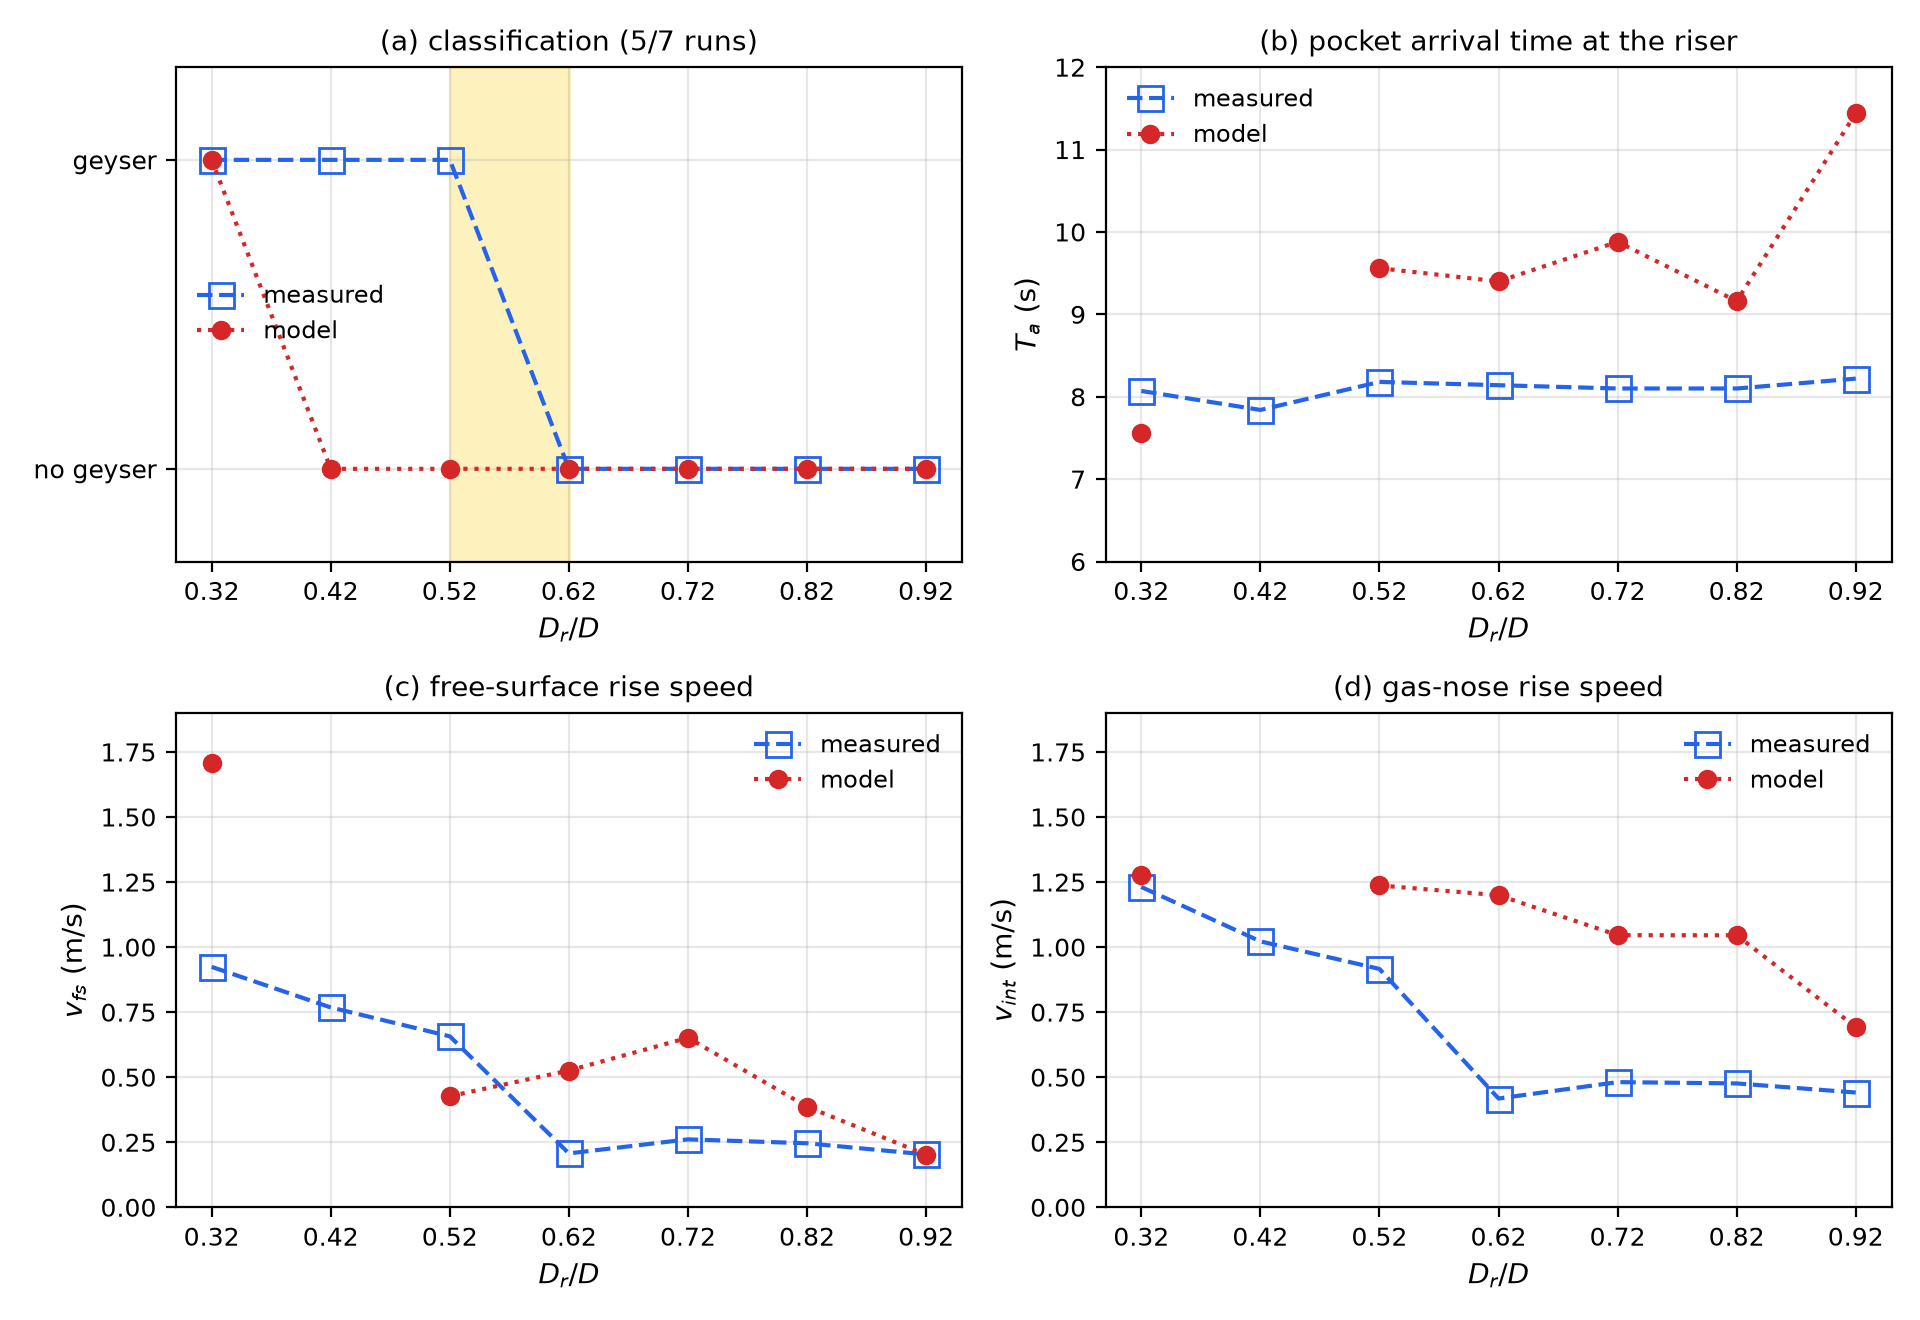
\includegraphics[width=\textwidth]{cong2017_bh_series.png}
\caption{算例组 2，\cite{cong2017} Series B：实测与计算的
(a) 喷发分类，(b) 气囊到达竖管时间，(c) 水面平均上升速度，(d) 气核前端平均上升速度，
均以竖管--管道直径比 $D_r/D$ 为横轴。}
\label{fig:cong_bh}
\end{figure}

图~\ref{fig:cong_signature} 给出两个签名工况的细节。B-H1（$D_r/D=0.32$）中，释放的
气囊在 $7.56$~s 到达（实测 $8.07$~s），入侵的气体以两次涌动脉冲顶托水面，供水管道
逆流的受阻将气囊压缩至 $1.71\,H_0$（周期平均，文献报告约 $1.9\,H_0$）而喷出水柱——
水面到顶时气核前端仍在其下，即喷发签名。B-H6（$D_r/D=0.82$）中同样的释放输送同样的
气囊，但宽竖管以温和顶托将水面推至 $0.78$~m，气囊排出而不喷发，到达后其压力从未超过
$1.02\,H_0$。管端压力的分支分化——因仅 $D_r$ 改变、是试验最干净的受控对照——在符号与
次序上被复现，但两者水平均被低估（$1.4\,H_0$ 的不喷发隆起被漏掉，因水库供水布置下计算
的水面抬升被低估，见第~\ref{sec:discussion}~节）。

\begin{figure}[htbp]
\centering
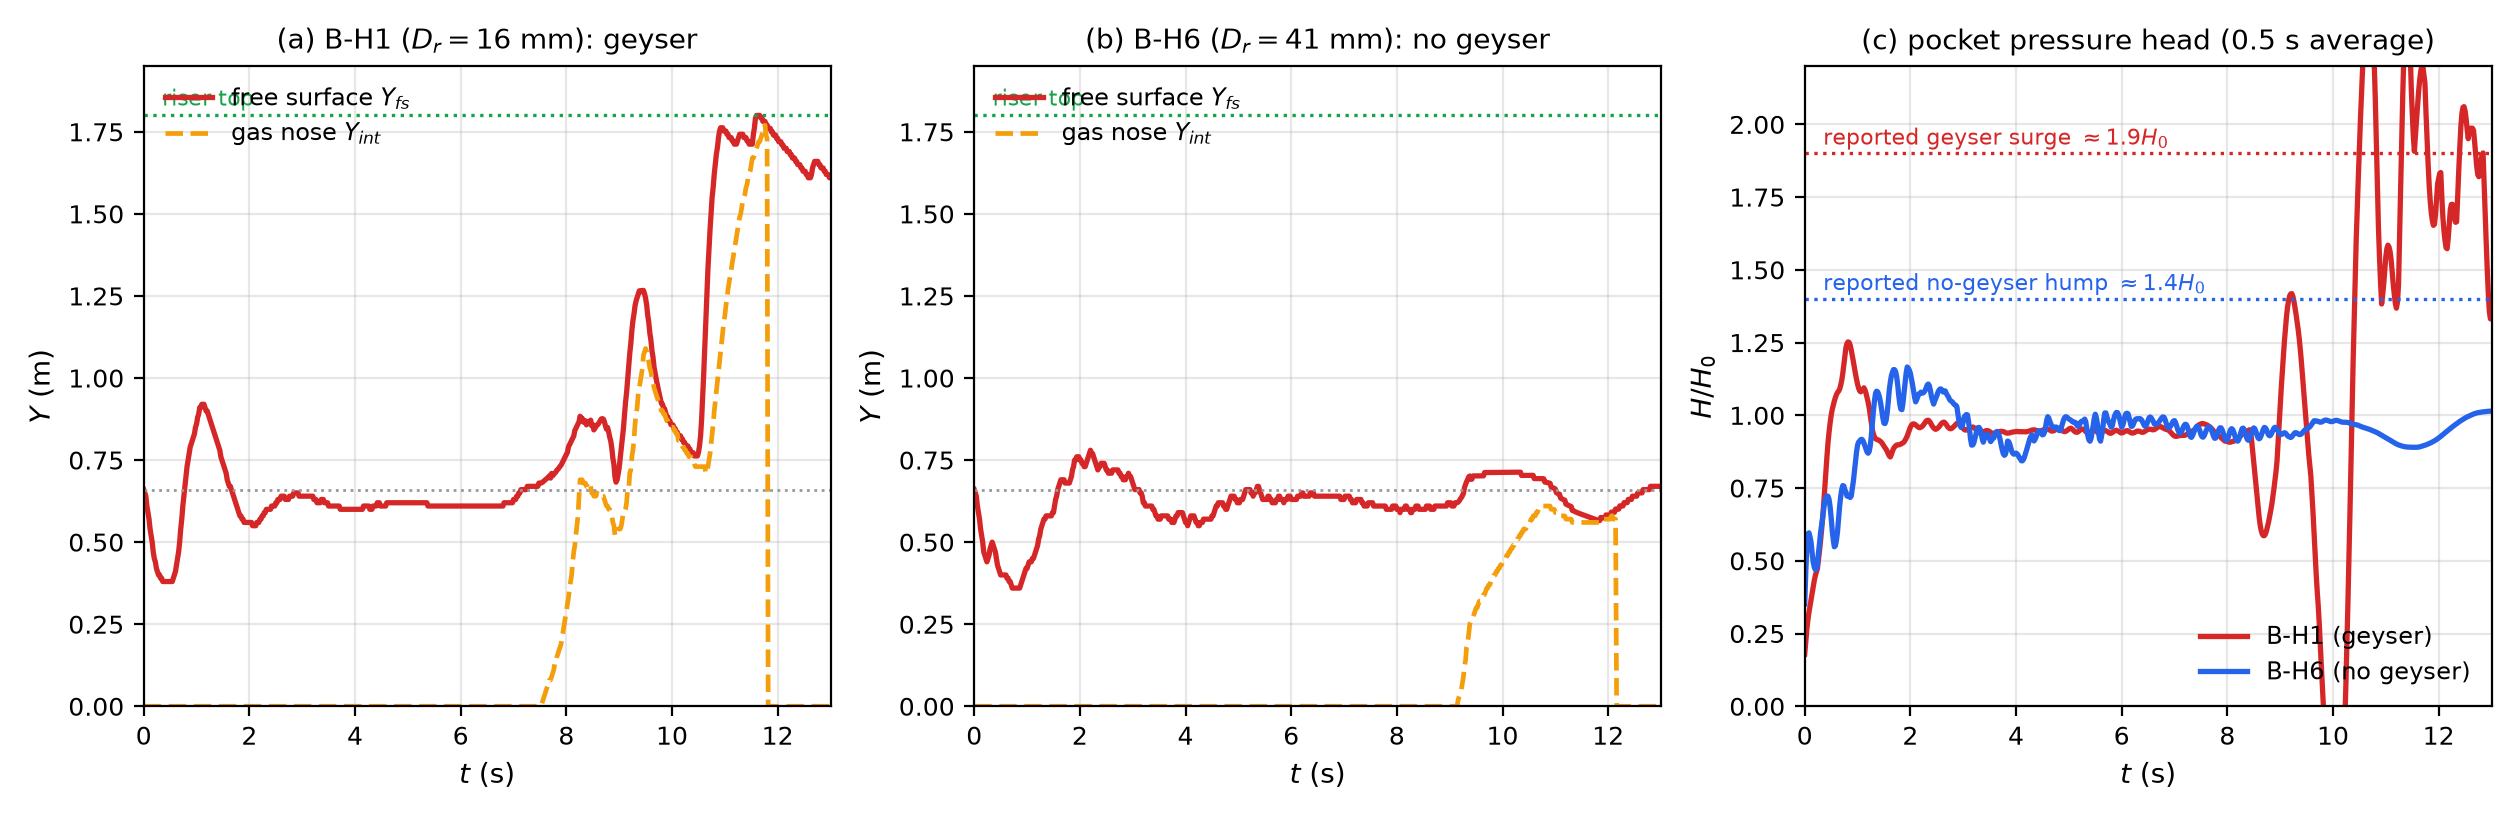
\includegraphics[width=\textwidth]{cong2017_signature.png}
\caption{算例组 2，\cite{cong2017} 签名工况（全同步耦合）：(a) 喷发工况 B-H1
（$D_r=16$~mm）计算的竖管自由水面与气核前端轨迹；(b) 不喷发工况 B-H6（$D_r=41$~mm）
同图；(c) 两工况计算的气囊压头（$0.5$~s 平均）与文献报告峰值水平对比（喷发涌峰
$\approx1.9\,H_0$；不喷发隆起 $\approx1.4\,H_0$）。}
\label{fig:cong_signature}
\end{figure}

\subsubsection{与试验判据的分支地图对比}
\label{sec:tests:cong2017:map}

图~\ref{fig:cong_map} 在判据平面 $(D_r/D,\ V^{*}_{air})$ 上给出 63 构型扫描。每个
构型是一次完整的全同步模拟，在不知晓式~(\ref{eq:cong_criterion}) 的前提下分类；判据线
仅作对照绘出。模型分类与试验判据在 63 个构型中的 39 个上一致，且 24 处分歧严格单向：
每一处都是判据判喷、模型判不喷。无一例假阳性——模型判喷的构型全部落在判据的喷发区内，
不喷发半平面 $D_r/D>0.62$ 全部分类正确，小气量区 $V^{*}_{air}<3.42$ 亦然。误判集中于
中等直径（$D_r/D=0.42$--$0.62$）与大气囊体积（$L_0\ge1.2$~m）的组合，那里计算水面被
顶托至 $1.0$--$1.6$~m 但未及 $1.8$~m 管顶；24 处中有 7 处已到管顶 $0.45$~m 以内。此
模式即 Series-B 顶托不足偏差在参数平面上的延伸：模型抓住了分支边界的物理结构——两个
端元与``喷发须同时满足细竖管\emph{与}相对大气囊体积''的交互取向——但把喷发阈值置得
偏保守，在过渡带低估喷发。对筛查用途而言偏差方向很关键：当前冻结模型在边界附近朝漏报
喷发出错，而非误报。

\begin{figure}[htbp]
\centering
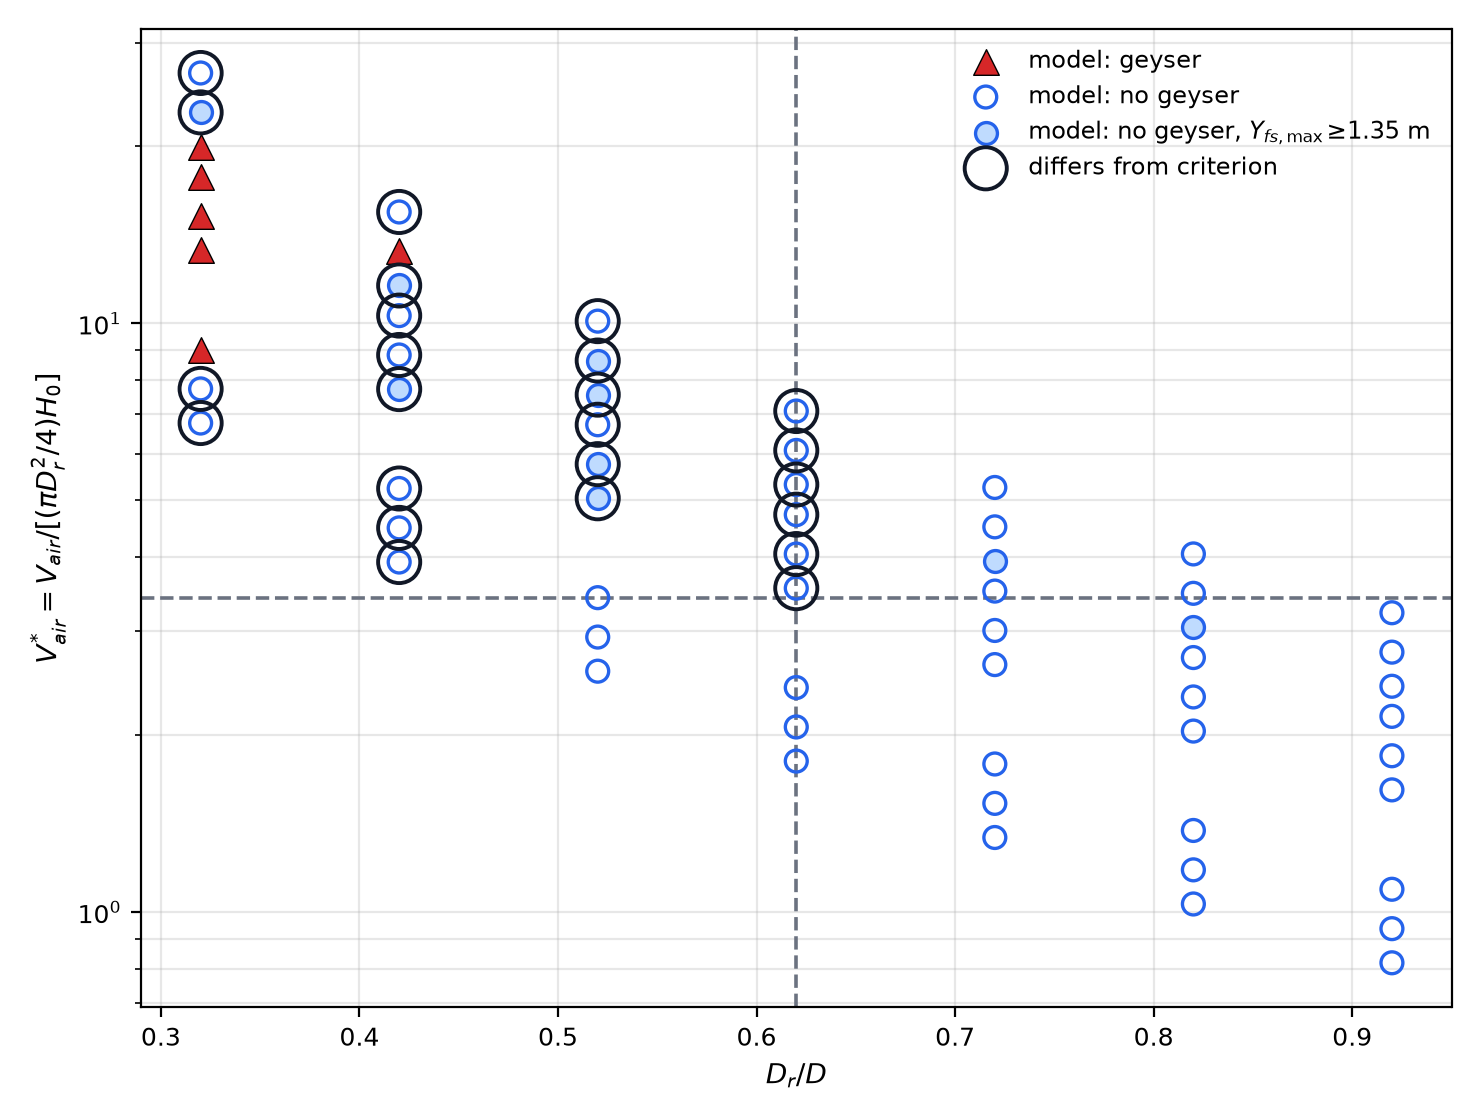
\includegraphics[width=0.85\textwidth]{cong2017_criterion_map.png}
\caption{算例组 2：覆盖 \cite{cong2017} 试验参数范围（$D_r=16$--$46$~mm，
$L_0=0.61$--$1.8$~m，$H_0=0.66$--$0.88$~m）的 63 个构型的模型喷发分类，每个均为一次
全同步模拟，绘于式~(\ref{eq:cong_criterion}) 的判据平面。实心三角：模型喷发；空心圆：
模型不喷发（浅色实心圆：水面到管顶 $0.45$~m 以内）；黑圈：与判据分歧；虚线：判据阈值
$D_r/D=0.62$ 与 $V^{*}_{air}=3.42$。模型在 63 个构型中的 39 个上一致；全部 24 处分歧
均为判据判喷/模型判不喷，无一例假阳性。}
\label{fig:cong_map}
\end{figure}

\FloatBarrier

\subsection{算例组 3：交汇室上方竖井中的雨水喷发（Liu、Shao 与 Zhu，2020）}
\label{sec:tests:liu2020}

\subsubsection{装置与一维复合域表示}
\label{sec:tests:liu2020:setup}

\cite{liu2020} 的装置为 Edmonton 27~m 深跌水井的 1:20 缩尺模型：上游管
5.80~m（$D=0.20$~m，坡度 1:100）、透明交汇室
$0.30\times0.30\times0.45$~m（至下游管底的落差为 0.18~m）和下游管
5.95~m（$D_d=0.28$~m）。交汇室顶盖中心安装直径 $d_r=0.06$~m、高
1.22~m、顶部通大气的竖管。进口为流量阶跃 $Q_0\to Q_1$，阀门开启时间
$T_v\approx0.4$~s。压力传感器 PT1--PT4 分别监测竖管、交汇室顶盖
（PT2，本文的主要基准点）、交汇室底板和上游管顶。

本文计算三个构型，均使用算例组 1--2 的同一冻结求解器。水平段表示为一个复合一维域：
上游管、交汇室和下游管在交汇处通过内部动量面连接；竖管水柱则表示为与顶盖压力点耦合
的刚性水柱常微分方程。该表述仍是降阶的一维模型：交汇室内三维掺混、交汇室气口处的
气塞排放，以及晚期工况中压缩气囊沿上游管顶抵达交汇室的过程，尚未在配套两流体/RTRP
框架的同等细节层级上解析；这些限制在下文对应结果处明确标出。

\subsubsection{分支对 A2/B3：仅改变下游边界即翻转结果}
\label{sec:tests:liu2020:AB}

A2 与 B3 使用相同的进口阶跃（$Q_0=20$、$Q_1=100$~L/s），只改变下游尾水：
A2 排向明渠（堰控，$h_d/D_d=1/4$），B3 初始满管且尾门淹没。试验中 A2 从不喷发，
而 B3 每次重复均产生一次单射流喷发（\cite{liu2020} 图~5）。

模型不重新调参即复现这一分支翻转。A2 的竖管水柱始终低于管顶：
$h_{r,\max}=0.47$~m，而竖管高 1.22~m；交汇室稳态压力也与数字化图~3 相符，
PT3 为 5.26~kPa（试验 4.99~kPa，模型相对高约 $5\%$），PT2 为 1.80~kPa
（试验 2.15~kPa，模型相对低约 $16\%$）。其中竖管静水头由复合域计算自然产生，
并非作为边界条件预设。

B3 的计算水面到达竖管顶并发生溢流。喷发时刻接近试验：PT2 峰值出现在
$1.68$~s，试验为 $1.47$~s；但冻结配置采用的弹性支路波速 $a_{wh}=40$~m/s
使短时压缩峰值欠分辨，PT2 峰值仅 31~kPa，而试验为 55~kPa（低估 $44\%$）。
将波速提高至 $80$~m/s 的敏感性计算给出 63.5~kPa，说明峰值差异主要随声学波速
变化，而非源于缺失的分支特定闭合。计算射流高度 $h=2.17$~m 落在
\cite{liu2020} 图~7(a) 的试验回归线
$h=0.694\,P_{\max}/\rho g+0.309$~m（$R^2=0.97$）上。

\begin{figure}[htbp]
\centering
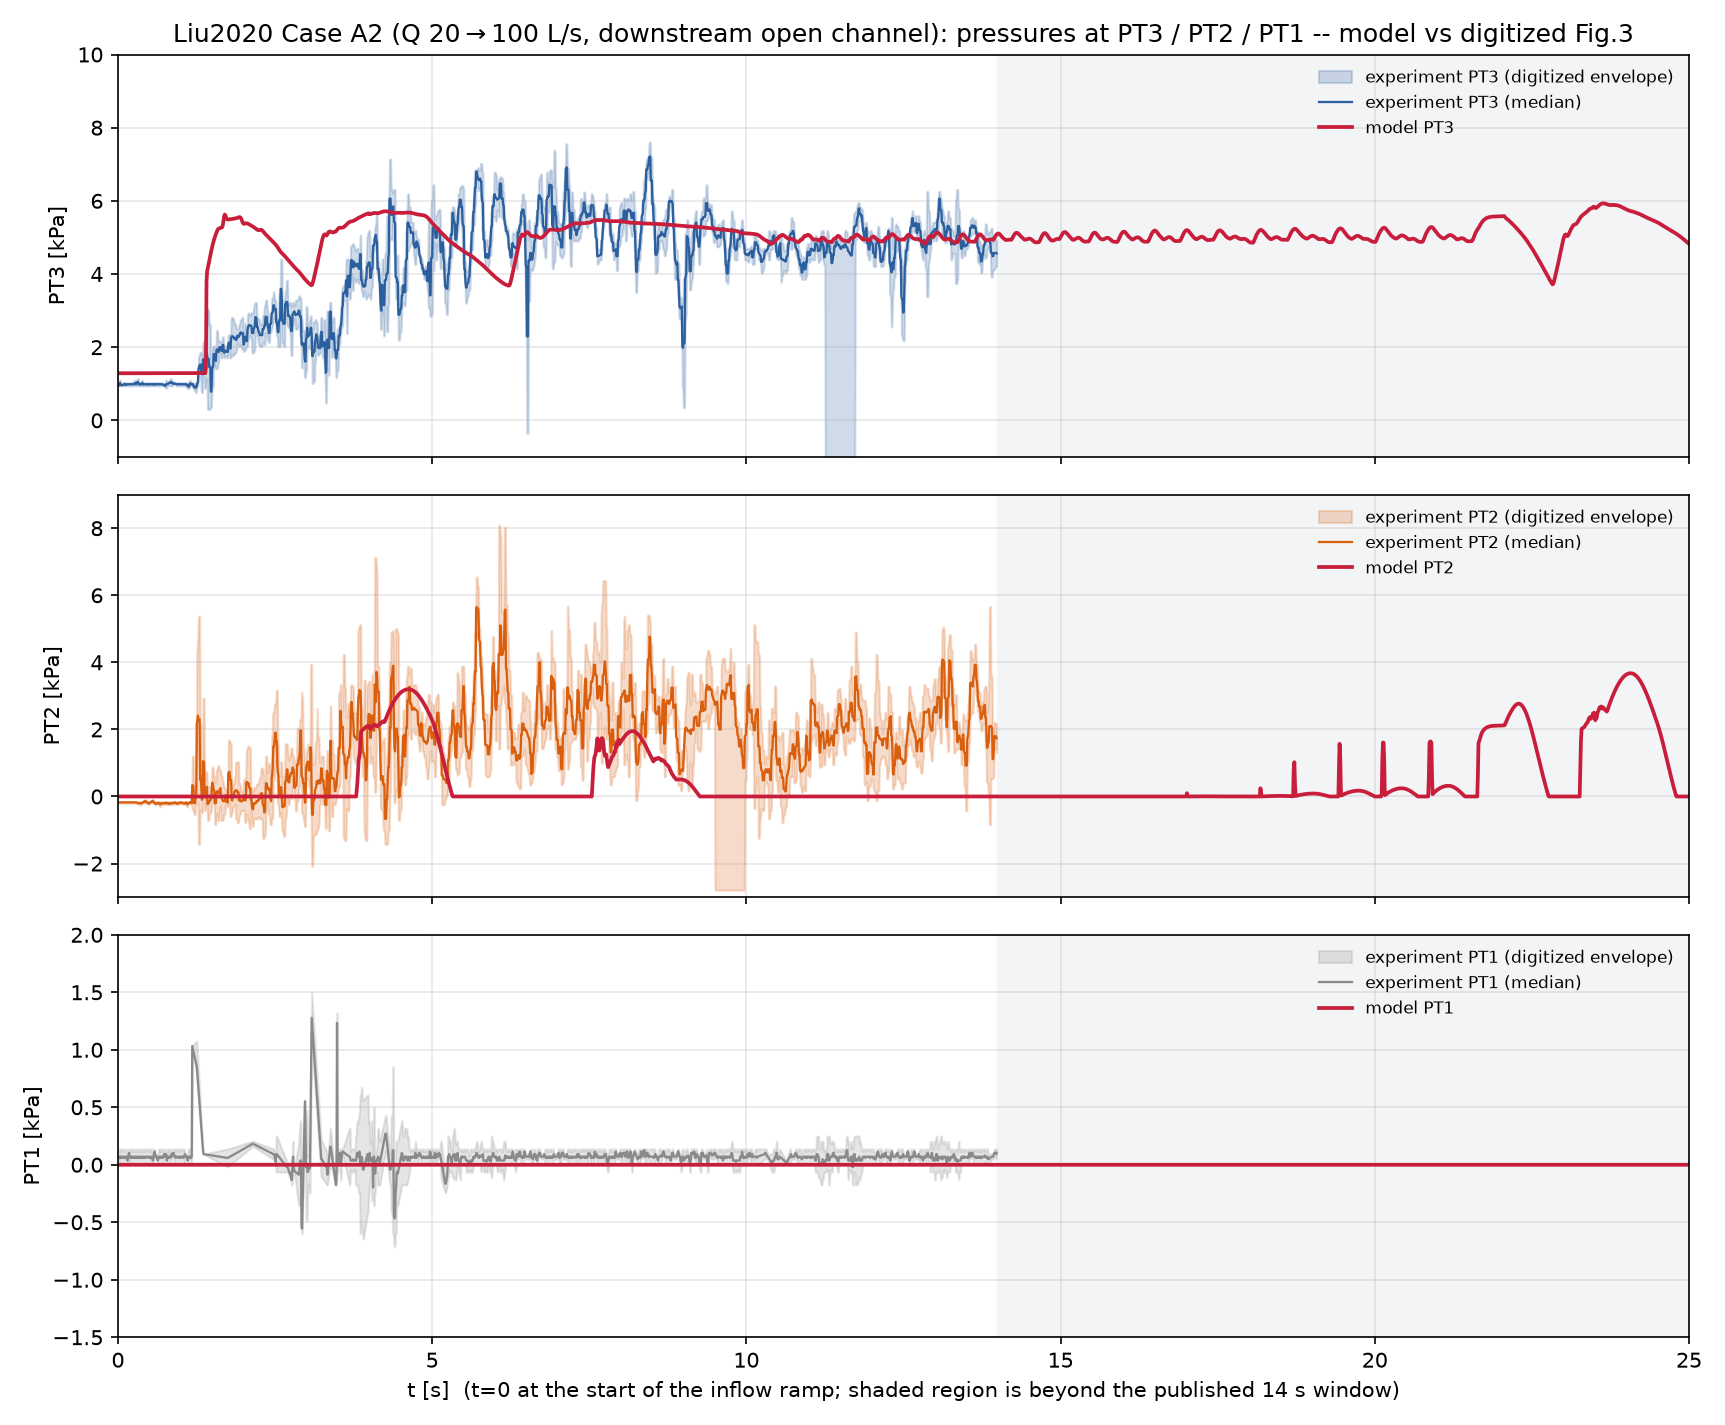
\includegraphics[width=\textwidth]{liu2020_a2_pressure.png}
\caption{工况 A2（$Q$: 20$\to$100~L/s，下游明渠）：交汇室与竖管压力时程。
蓝色：从 \cite{liu2020} 图~3 数字化的 PT2/PT3 试验结果；红色：本文模型。}
\label{fig:liu_a2_pressure}
\end{figure}

\begin{figure}[htbp]
\centering
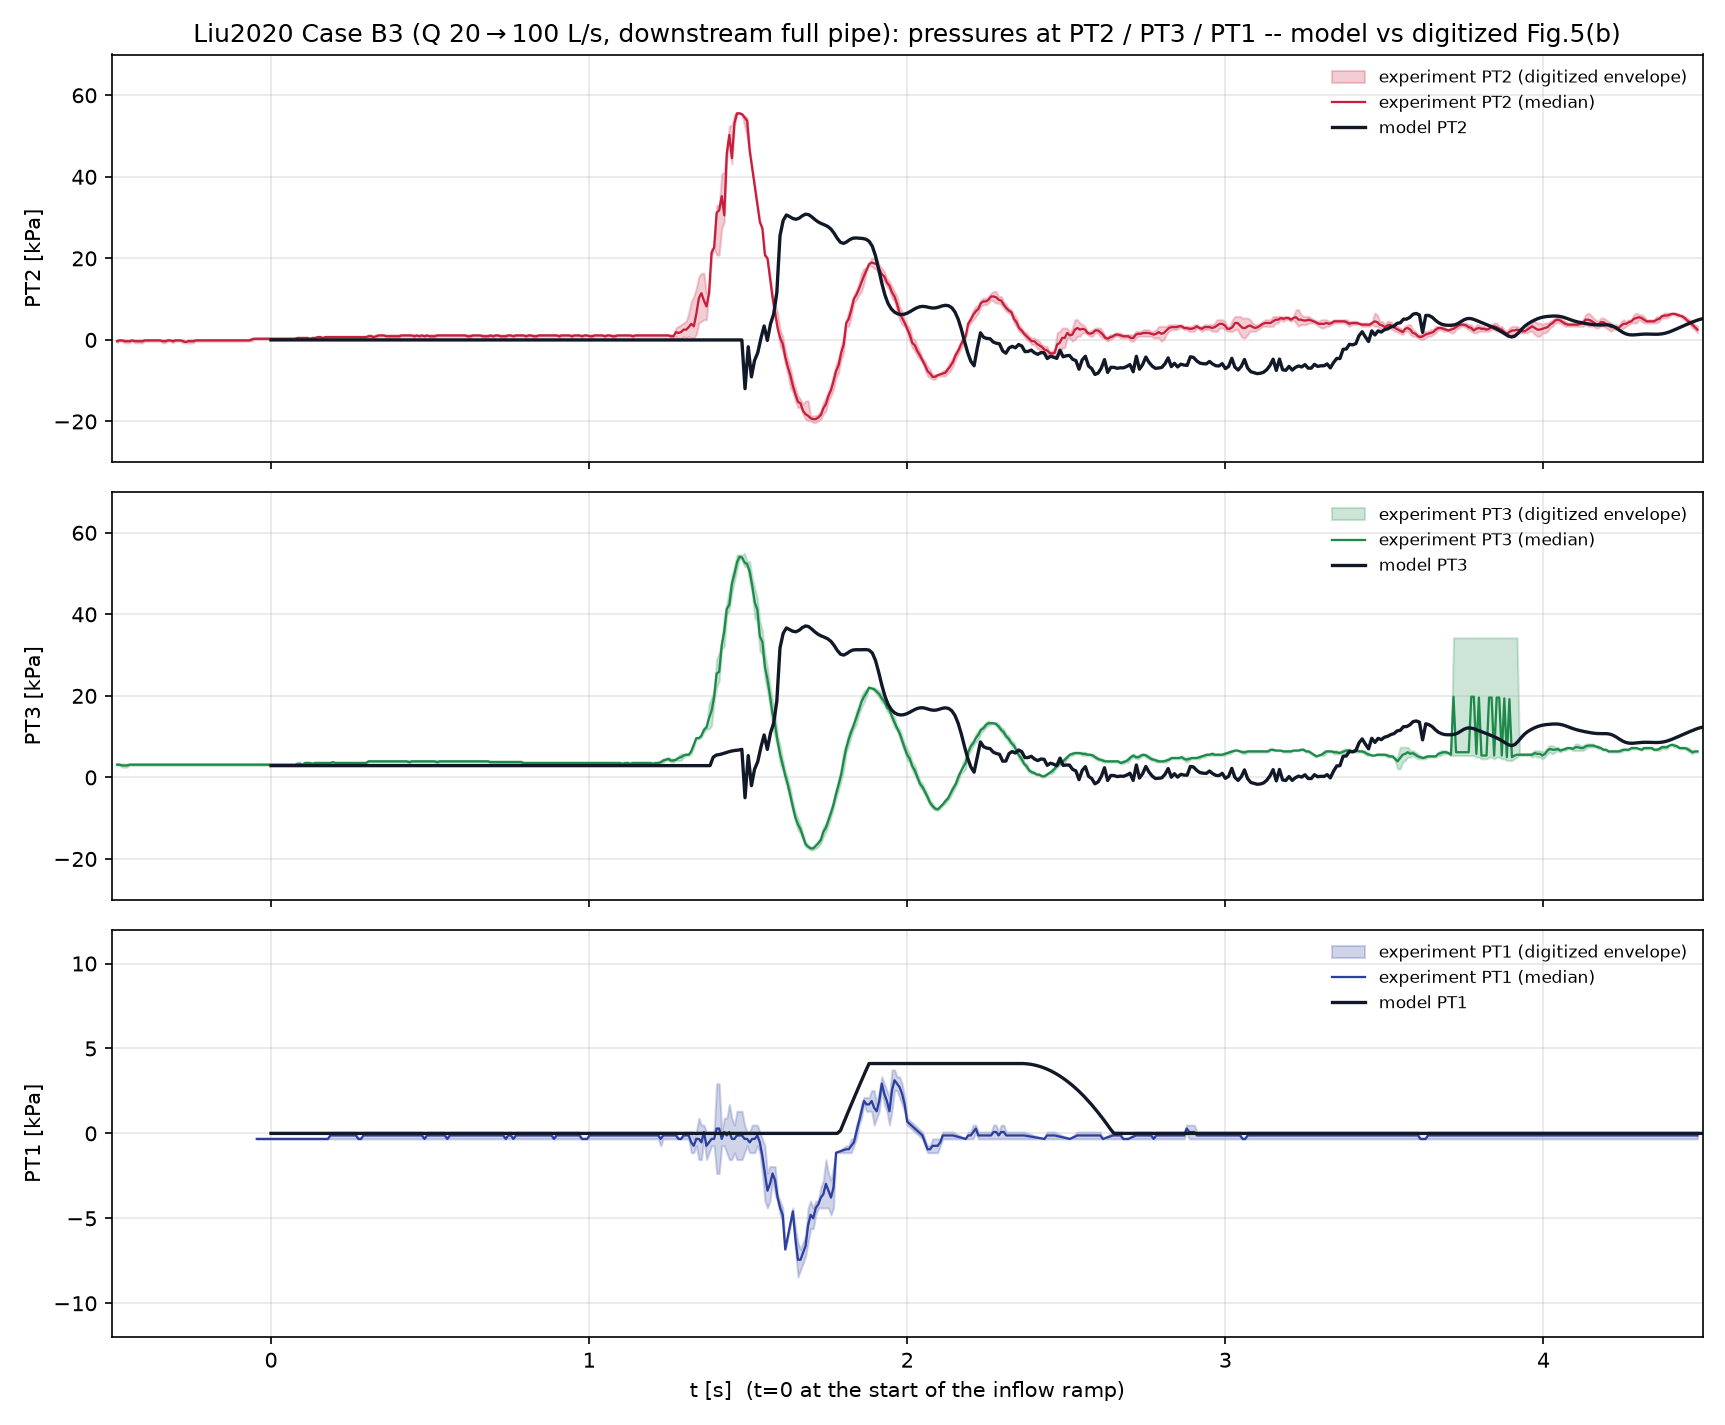
\includegraphics[width=\textwidth]{liu2020_b3_pressure.png}
\caption{工况 B3（$Q$: 20$\to$100~L/s，下游满管）：PT1--PT3 压力时程。
蓝色：从 \cite{liu2020} 图~5(b) 数字化的试验结果；红色：本文模型。模型选中
喷发分支，但冻结波速 $a_{wh}=40$~m/s 对短时压缩峰值存在声学欠分辨。}
\label{fig:liu_b3_pressure}
\end{figure}

\begin{figure}[htbp]
\centering
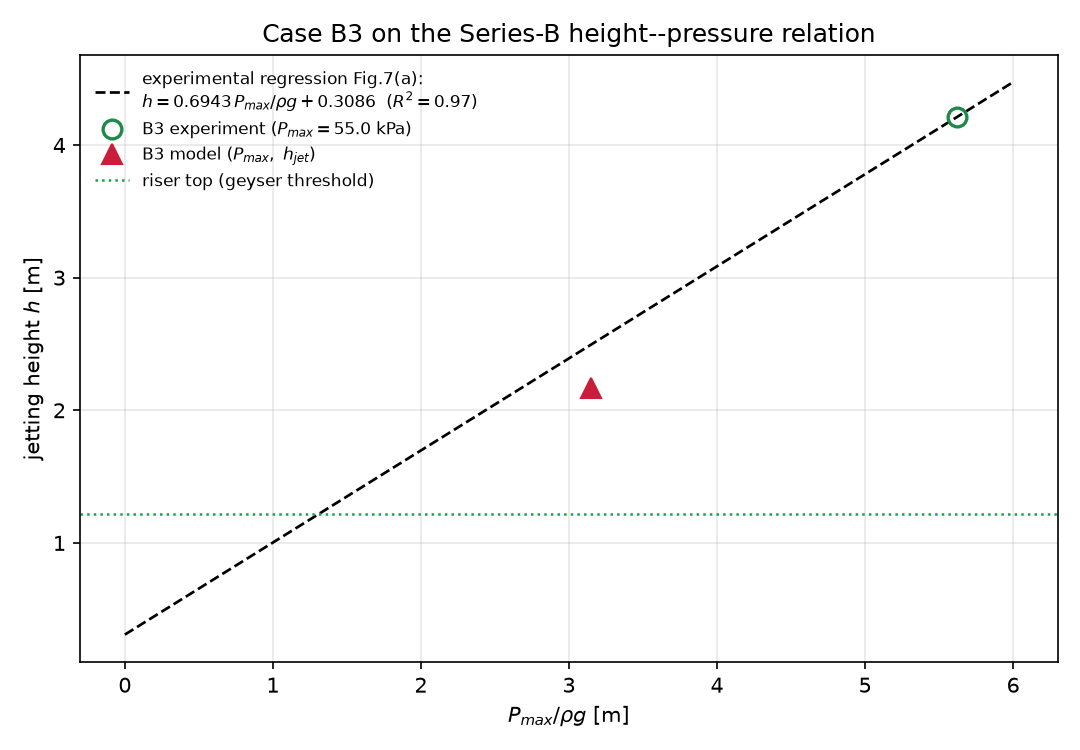
\includegraphics[width=0.72\textwidth]{liu2020_b3_h_pmax.png}
\caption{工况 B3 在 \cite{liu2020} 图~7(a) 的喷发高度--峰值压力图上的位置。
空心符号：试验工况族；红色实心圆：本文模型
（$h=2.17$~m，$a_{wh}=40$~m/s 时 $P_{\max}=31$~kPa）。}
\label{fig:liu_b3_h_pmax}
\end{figure}

\subsubsection{工况 C9：瞬变驱动喷发与解析质量振荡模型}
\label{sec:tests:liu2020:C9}

工况 C9（$Q_0=25\to Q_1=40$~L/s，下游满管，竖管初始水柱
$h_{r0}=0.30$~m；试验中上游管顶存在密闭气楔）是文献详细分析的两阶段工况：
气囊在 $t\approx6.46$~s 抵达交汇室之前，第 1--2 次喷发由水力瞬变驱动；
其后的第 3--8 次喷发由气囊驱动，超出当前降阶求解器的物理范围。

第一阶段对比采用全水计算变体，与 \cite{liu2020} 式~(7) 的假设一致；密闭气囊变体
仅保留为气体缓冲效应的定性检验。交汇室顶盖处的解析水头为
\begin{equation}
H_s(t)=h_{r0}+\frac{L_d}{gA_d}\frac{\mathrm{d}Q_u}{\mathrm{d}t}
\left(1-\cos\frac{2\pi t}{T}\right),
\qquad
T=2\pi\sqrt{\frac{L_d A_r}{gA_d}+\frac{h_{r0}}{g}},
\label{eq:liu_eq7}
\end{equation}
对 C9 得 $T=1.52$~s。

图~\ref{fig:liu_c9_phase1} 将数字化的文献图~9 PT2 记录（转换到交汇室顶盖水头基准）
与式~(\ref{eq:liu_eq7}) 及全水模型在最初 5~s 内进行对比。首个峰值的时刻和幅值均得到
复现：试验为 10.69~kPa、$t=0.50$~s，模型为 11.5~kPa、$t=0.54$~s；
试验水面于 0.73~s 到达竖管顶，模型为 0.93~s。振荡周期则为试验 1.45~s、
模型 1.13~s、式~(\ref{eq:liu_eq7}) 1.52~s；模型比试验偏快，符合刚性一维尾门
耦合偏硬的特征。第一轮瞬变之后的稳态压力在约 $20\%$ 内一致，PT2 终值为试验
8.79~kPa、模型 10.6~kPa。密闭气囊变体定性复现了首峰的推迟与削弱，但在约
4~s 后因气楔在降阶气体模型中持续压缩而漂移；该阶段不作定量结论。

\begin{figure}[htbp]
\centering
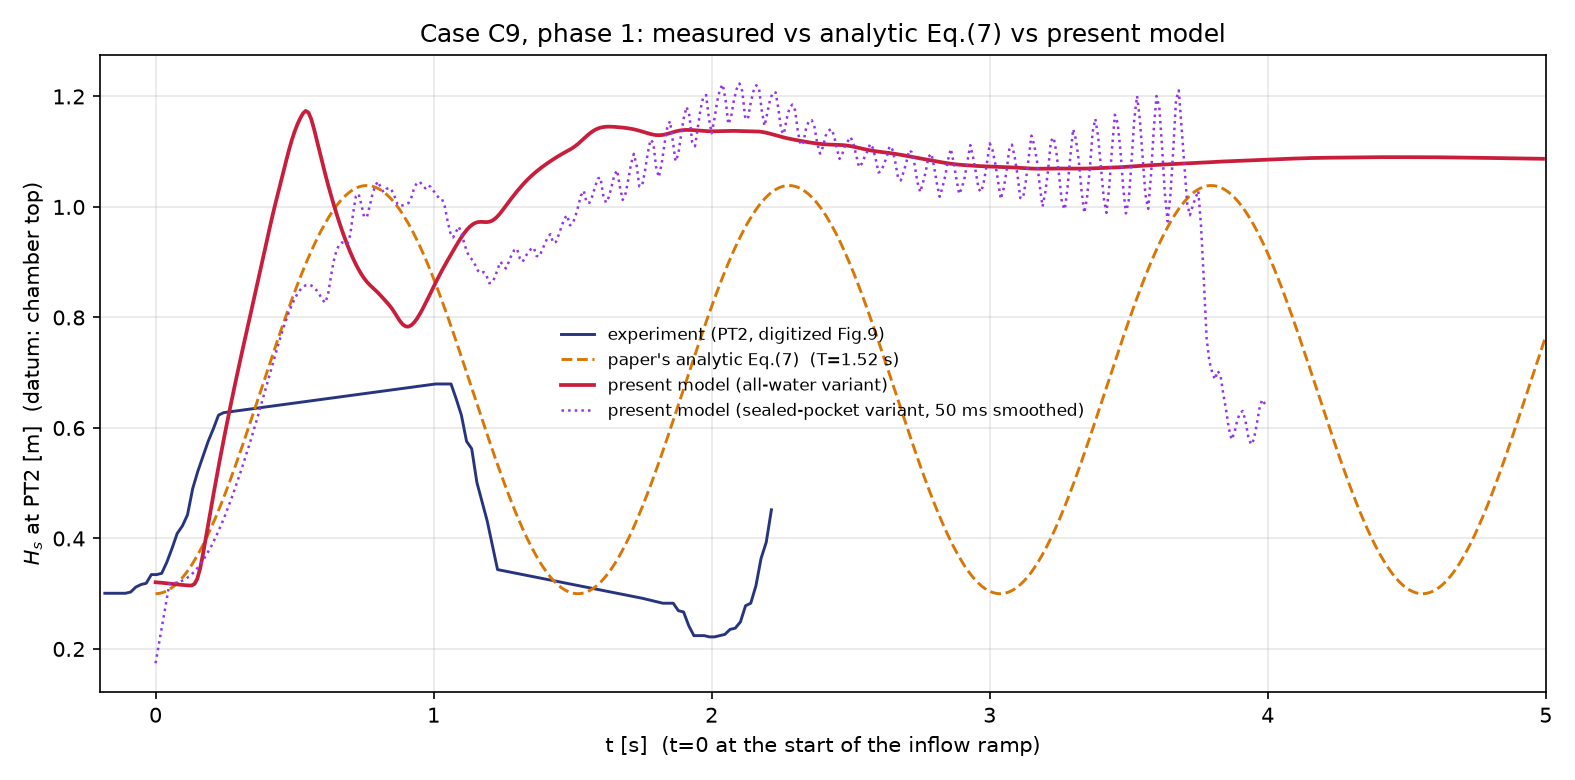
\includegraphics[width=\textwidth]{liu2020_c9_phase1.png}
\caption{C9 第一阶段（$t<5$~s）：交汇室顶盖基准下的 PT2 水头 $H_s$。
蓝色：从 \cite{liu2020} 图~9 数字化的试验值；橙色虚线：文献式~(7)；
红色：本文全水模型；紫色点线：密闭气囊变体（50~ms 平滑）。气囊于
$t\approx6.5$~s 抵达后的气囊驱动喷发未计算。}
\label{fig:liu_c9_phase1}
\end{figure}

\begin{figure}[htbp]
\centering
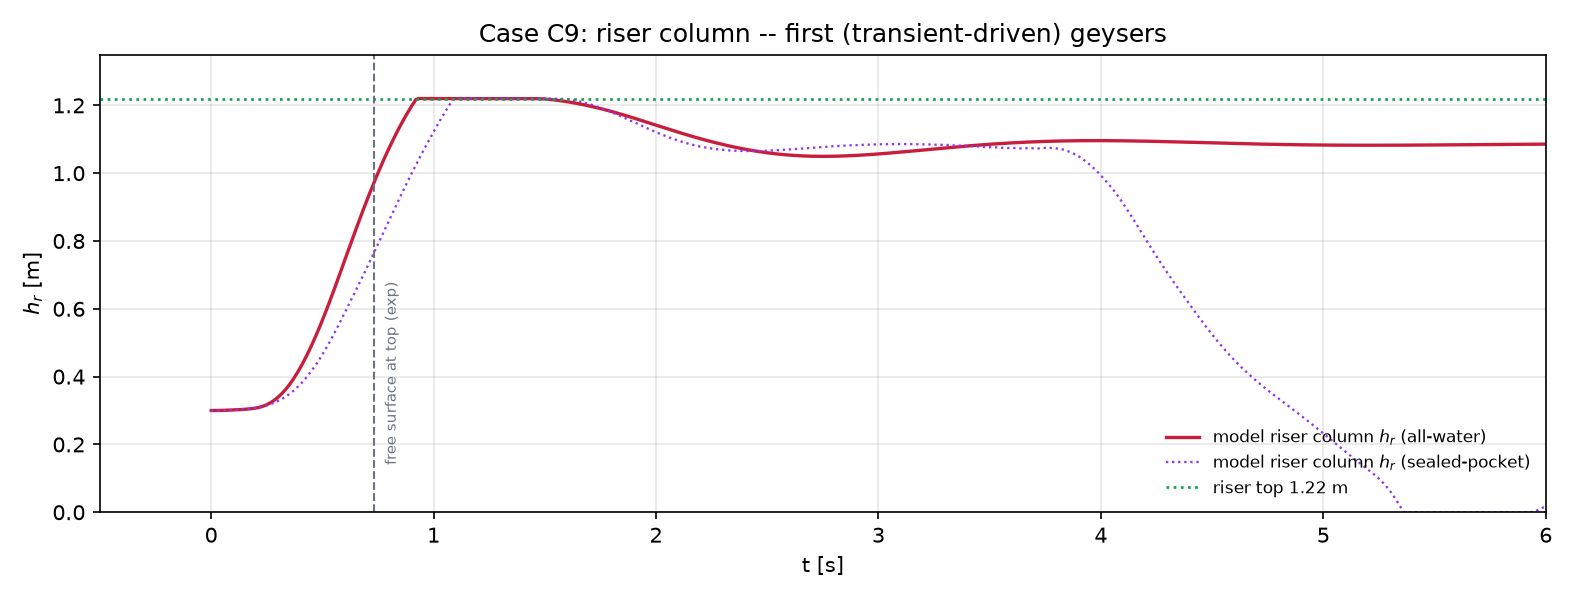
\includegraphics[width=\textwidth]{liu2020_c9_riser.png}
\caption{C9 竖管水柱高度 $h_r$：全水变体（实线）与密闭气囊变体（点线）。
竖虚线标记试验第一阶段中水面首次到达竖管顶的时刻。}
\label{fig:liu_c9_riser}
\end{figure}

\begin{table}[htbp]
\centering
\caption{算例组 3 主要指标汇总。声学峰值使用冻结配置
$a_{wh}=40$~m/s；各工况之间不重新调整系数。}
\label{tab:liu_summary}
\resizebox{\textwidth}{!}{%
\begin{tabular}{lccc}
\toprule
指标 & A2（不喷发） & B3（喷发） & C9 第一阶段 \\
\midrule
是否喷发（模型/试验） & 否 / 否 & 是 / 是 & 是 / 是 \\
PT2 稳态或峰值 [kPa] & $1.80$ / $2.15$ & $31$ / $55$ & $11.5$ / $10.7$ \\
峰值或到顶时刻 [s] & --- & $1.68$ / $1.47$ & $0.54$ / $0.50$ \\
水面到达竖管顶 [s] & --- & $\approx1.65$ & $0.93$ / $0.73$ \\
振荡周期 [s] & $0.30$（PT2--PT3） & --- & $1.13$ / $1.45$ \\
\midrule
\multicolumn{4}{l}{\footnotesize 注：除明确标注外，含斜线单元格均为模型值 / 试验值。}\\
\bottomrule
\end{tabular}
}
\end{table}

综合三个工况，复合域表述把算例组 1--2 的冻结求解器延伸到了具有原型背景的交汇室几何：
仅改变下游边界的分支对 A2/B3，以及 C9 第一阶段的瞬变质量振荡喷发，均在分支判别、
时序和非声学主导的幅值层面得到复现。本算例组的主要残余是：冻结弹性波速对短时压缩峰值
的欠分辨，以及气囊抵达交汇室后因缺少气囊输运与气室排放物理而有意划定的范围边界。

\FloatBarrier

% ======================================================================
\section{讨论}
\label{sec:discussion}

\subsection{框架解析了什么}

第~\ref{sec:tests}~节的对比表明：在竖井与管道中守恒气体质量与动量、对截留气囊按解析
囊体积用状态方程闭合的一维公式，足以在不引入分支特定输入的情况下选出喷发分支。宽塔
工况中，泄放路径——气囊经塔泄放叠加井口逆向交换——确定了一个压力平台，其水平与
时长由气囊体积与塔内静水柱控制；二者均得以复现，因为它们来自守恒律而非标定闭合。
宽塔中的界面爬升速度同样在不输入任何漂移通量关系的情况下复现于泰勒气泡尺度，因为
气核在解析液柱中的浮升本就是两流体解的一部分。

Tests A 与 B 之间的分支判别由塔径通过两个相互竞争、且均被模型解析的速率控制：气囊向
塔底泄气的速率，与塔通过其水柱传气并在井口排出的速率。宽塔中水柱以适度的水面抬升传气；
细塔中同样的泄气体积把水柱直接顶至井口。这正是~\cite{vasconcelos2011}~在试验上识别的
机制，此处它从计算状态中自然涌现。

算例组 2 检验这一判别能否推广到单一装置之外，答案是结构性的而非均匀的。在
\cite{cong2017} 参数范围的 63 构型扫描上（以相同的冻结求解器计算、不知晓试验判据），
模型精确复现了分支边界的两个端元——每个宽竖管构型（$D_r/D>0.62$）与每个小气量
构型（$V^{*}_{air}<3.42$）均排气不喷发，最细竖管配大气囊则喷发——并复现了判据的交互
取向，因为两个阈值都源于同一被解析的竞争：气囊必须以快于竖管透过水柱排气的速率
（直径条件）维持其对收缩水柱的超压（体积条件）。然而在过渡带内模型偏保守：63 个中有
24 个被判据标为喷发的构型，被算成强但未及管顶的水柱抬升（$1.0$--$1.6$~m 对 $1.8$~m
管顶），对应的两个中等直径 Series-B 工况（B-H2、B-H3）也是 7 个高速摄像工况中仅有的
分类误判。全部分歧均为单向——没有任何被判据排除的构型在模型中喷发——故冻结配置朝漏报
边缘喷发出错，而非误报。

\subsection{已识别的局限}

已完成的算例组暴露出五项局限，均处于结点与闭合处理层面而非两流体公式本身，且与配套
论文~\cite{xue2026model}所列模型简化一致。

\emph{结点基准面。}算例组 1 的两个分支目前对井底耦合采用不同的高程基准：宽塔工况向
井底传递管底测压管水头，细塔工况传递管顶压力（竖井在管顶开孔，管顶比管底高一个管径）。
管顶基准是几何上正确的选择；在细塔中这一差别——至多 $\rho_l g D=0.15L$ 的虚假驱动
压头——决定了水柱是被钉在井口还是停在实测的准静态驻位。宽塔中该区别被含气水柱掩盖
（可见水位包含气泡持留的涌胀），管底耦合复现了量测；合并目标是一个跨井口携带竖向压力
分布的单一结点闭合，而非单一标量基准。

\emph{细井爬升闭合。}细塔的实测界面爬升（$V^{*}_{int}=1.43$，远超泰勒气泡尺度）只有
把与气囊连通的井内气体作为气囊供压的连通气核处理——井口流入抬升鼻端、通量受 Wallis
逆流淹没尺度约束——才得以复现。这两个要素使用文献常数（$C_w=0.9$）与几何填充水平，
不做逐工况拟合，但只在受驱区（$H_{a0}>Y_{fs,0}$ 且结点携气）激活；非受驱区保留弥散
气泡阻力路径。算例组 2 的``排气不喷发''工况中，受驱路径的供气使爬升以涌动脉冲呈现
（最速持续爬升 $0.7$--$1.2$~m/s），而实测为稳定的泰勒尺度上升（$0.42$--$0.48$~m/s）；
以当地气体通量为条件的竖直环状流卷吸闭合可统一两条路径并平滑脉冲。

\emph{管顶气穴提前抵塔。}算例组 1 的两个分支中，气相事件序列均以一致的偏移提前
（Test~A 为 $0.3$--$0.4$、Test~B 为 $0.3$--$0.6$ 个时间单位），而事件间隔正确。
本工作中识别并消除了前沿追踪交接中的一处离散偏差：气穴鼻端单元在区域平均层深的
$95\%$ 处即被释放给下一单元，使检测前沿以体积预算的 $95\%$ 推进，把输运偏置到
Benjamin 波速的 $1.09$ 倍；改为按完整体水平交接后，计算输运为 Benjamin 波速的
$0.96$ 倍，与实测中段管输运（$2.97$~m 历时 $5.9$~s）一致。残余偏移与手动蝶阀开启
的不确定度同量级：模型以 $0.25$~s 节流斜坡表示开阀，而试验仅报告``一秒内开启''，
该差异在两种塔尺度下折合 $0.3$--$0.9$ 个时间单位。由于偏移是刚体的，它不影响分支
判别与爬升运动学。

\emph{释放振荡阻尼。}两组算例中均可见的欠阻尼释放活塞振荡是系统的真实模态——气体
弹簧上的水柱——\cite{vasconcelos2011} 的装置示意图对其有明确标注；实验迹线约一个
时间单位内衰减，模型需数个。试验中的阻尼由阀门与联轴节处的三维掺混损失提供，常数
阀门与结点损失系数能捕捉均值，但不能捕捉逐周期的耗散。细塔中残存的振荡还使水柱在
释放摆动期间短暂溅至井口，随后才回落至准静态驻位；算例组 2 中同一简化把 B-H1 的喷发
射流削锐（事件速度 $1.71$ 对 $0.92$~m/s）。

\emph{水库供水布置下的体积中性口部交换。}T 型口部的倒瓶``咕咚''交换——气上、等体积水
下——是气体透过驻立水柱迁移时维持气囊压力的机制，也是 B-H1 喷发的关键：没有它，细竖管
气囊无法重建那道喷出水柱的过压。但在算例组 2 的水库供水布置中，同一交换又抵消了入侵
气体体积本应产生的一对一水柱抬升，且抵消随竖管变宽而增大：计算的 B-H6 水面抬升为
$+0.12$~m，实测 $+0.63$~m；在 63 构型扫描上，这一顶托不足正是过渡带单向误判的成因
（第~\ref{sec:tests:cong2017:map}~节）。对水库供水工况关闭该交换的做法已试并被否决：
它虽恢复宽竖管抬升，却在均衡排气阶段打开窄气囊的体积，其压力再也无法重建，B-H1 喷发
随之丢失。两分支对单一口部闭合提出相互冲突的需求；以口部当地逆流容量（而非体积中性）
计量该交换的表述，连同上面的卷吸闭合，是已识别的改进方向。

\subsection{本次验证的范围}

已完成的算例组覆盖三套装置、三类证据：单井双分支时程（算例组 1）、竖管--定水头
参数扫描分类（算例组 2）、原型背景交汇室的下边界分支对与 C9 瞬变振荡喷发
（算例组 3），均采用同一冻结求解器与全同步结点耦合。算例组 1 分支判别精确；
算例组 2 判据边界结构复现、过渡带单向保守（5/7、39/63）；算例组 3 中 A2/B3
仅换下游即翻转分支，C9 第一阶段首峰时刻与幅值贴近试验与 Eq.(7)，冲击峰与
气囊抵达后的喷发受冻结波速与降阶交汇室表述限制。三点限定：其一，Test~B 细井
闭合待与宽塔合并；其二，口部体积中性交换对算例组 2 两分支需求冲突；其三，
算例组 3 未解析气囊输运至交汇室及气室排气，更大尺度对比~\cite{muller2017}
仍待单独开展。

\section{结论}
\label{sec:conclusions}

本文将~\cite{xue2026model}的解耦两流体切割单元有限体积框架应用于实验室喷发试验：
竖井表示为旋转至竖直方向的同一套一维两流体系统，经结点损失闭合与水平管耦合。完成三组
算例，均从试验初始条件计算，不预设释放速率、不做逐工况拟合。

对 Vasconcelos 与 Wright \cite{vasconcelos2011} 的通风竖井试验，模型在不喷发与喷发
两个构型上均选对分支。不喷发分支复现了压力平台水平与时长、末段泄放衰减起始、最大
水面抬升与气水界面爬升速度。喷发分支复现了塔内水柱的喷发前准静态驻位（$0.84L$ 对
实测 $0.82L$）、管顶基准压力平台（$0.76$ 对 $0.76$）、试验每次重复观测到的喷发至
井口、界面与水面爬升速度（$V^{*}_{int}=1.19$ 对 $1.43$；$V^{*}_{fs}=0.42$ 对
$0.44$），以及气囊泄放时压头的``平台--骤降''形态；细井闭合由管顶基准井底耦合、
气囊供压气核与 Wallis 淹没限进气组成，只使用几何事实与文献尺度常数。剩余偏差为
气相事件时刻的整体提前（$0.3$--$0.6$ 个时间单位，与手动开阀时间的不确定度同量级）
与欠阻尼的释放振荡。

对 Cong、Chan 与 Lee \cite{cong2017} 的水平管/竖管试验，在同一冻结求解器与全同步
耦合下，模型复现了文献双参数喷发判据的分支结构：喷发端元 B-H1（压缩涌峰驱动至
$1.71\,H_0$）、整个不喷发半平面 $D_r/D>0.62$ 与小气量区，以及只有耦合的竖管--管道
计算才能产生的管端压力分支分化。误差是单向且保守的：两个中等直径 Series-B 工况与
63 构型中的 24 个试验喷发构型，被计算为强但未及管顶的水柱抬升，无一例假阳性；偏差
追溯至体积中性口部交换，两分支对该闭合的冲突需求是首要改进目标。

对 Liu、Shao 与 Zhu \cite{liu2020} 的交汇室试验，复合一维表述下复现了 A2/B3
下游边界分支翻转，B3 喷发高度落在试验 $h$--$P_{\max}$ 回归线上（峰压受
$a_{wh}=40$~m/s 声学限制），C9 第一阶段与试验及 Eq.(7) 在首峰时刻与幅值上一致；
气囊抵达交汇室后的喷发声明为范围外。

上述结果支持将守恒气相的一维两流体模型用于系统尺度喷发筛查——其首要问题是分支判别
与排气行为而非射流细节——并把结点与卷吸闭合确定为喷发分支定量改进的目标。

\section*{数据可用性声明}

第~\ref{sec:tests}~节结果所用的冻结求解器快照、数字化试验曲线与对比脚本可向通讯作者
索取。

% ======================================================================
\begin{thebibliography}{00}
% 参考文献保留英文原文（与英文版一致，按引用顺序）。

\bibitem{wright2011note}
S.J.~Wright, J.W.~Lewis, J.G.~Vasconcelos,
Geysering in rapidly filling storm-water tunnels,
J.~Hydraul.~Eng. 137 (1) (2011) 112--115,
doi:10.1061/(ASCE)HY.1943-7900.0000245.

\bibitem{vasconcelos2011}
J.G.~Vasconcelos, S.J.~Wright,
Geysering generated by large air pockets released through water-filled
ventilation shafts,
J.~Hydraul.~Eng. 137 (5) (2011) 543--555,
doi:10.1061/(ASCE)HY.1943-7900.0000332.

\bibitem{cong2017}
J.~Cong, S.N.~Chan, J.H.W.~Lee,
Geyser formation by release of entrapped air from horizontal pipe into
vertical shaft,
J.~Hydraul.~Eng. 143 (9) (2017) 04017039,
doi:10.1061/(ASCE)HY.1943-7900.0001332.

\bibitem{muller2017}
K.Z.~Muller, J.~Wang, J.G.~Vasconcelos,
Water displacement in shafts and geysering created by uncontrolled air
pocket releases,
J.~Hydraul.~Eng. 143 (10) (2017) 04017043,
doi:10.1061/(ASCE)HY.1943-7900.0001362.

\bibitem{liu2020}
L.~Liu, W.~Shao, D.Z.~Zhu,
Experimental study on stormwater geyser in vertical shaft above junction
chamber,
J.~Hydraul.~Eng. 146 (2) (2020) 04019055,
doi:10.1061/(ASCE)HY.1943-7900.0001660.

\bibitem{zhang2022}
Y.~Zhang, Y.~Chen, S.~Qian, H.~Xu, J.~Feng, X.~Wang,
Experimental study on geysers in covered manholes during release of air
pockets in stormwater systems,
J.~Hydraul.~Eng. 148 (5) (2022) 06022003,
doi:10.1061/(ASCE)HY.1943-7900.0001978.

\bibitem{qian2020}
Y.~Qian, D.Z.~Zhu, L.~Liu, W.~Shao, S.~Edwini-Bonsu, F.~Zhou,
Numerical and experimental study on mitigation of storm geysers in
Edmonton, Alberta, Canada,
J.~Hydraul.~Eng. 146 (3) (2020) 04019069,
doi:10.1061/(ASCE)HY.1943-7900.0001684.

\bibitem{zhouprosperetti2019}
G.~Zhou, A.~Prosperetti,
Violent expansion of a rising Taylor bubble,
Phys.~Rev.~Fluids 4 (7) (2019) 073903,
doi:10.1103/PhysRevFluids.4.073903.

\bibitem{leon2018}
A.S.~Le\'{o}n, I.S.~Elayeb, Y.~Tang,
An experimental study on violent geysers in vertical pipes,
J.~Hydraul.~Res. 57 (3) (2019) 283--294,
doi:10.1080/00221686.2018.1494052.

\bibitem{chan2018}
S.N.~Chan, J.~Cong, J.H.W.~Lee,
3D numerical modeling of geyser formation by release of entrapped air from
horizontal pipe into vertical shaft,
J.~Hydraul.~Eng. 144 (3) (2018) 04017071,
doi:10.1061/(ASCE)HY.1943-7900.0001416.

\bibitem{vasconcelos2006}
J.G.~Vasconcelos, S.J.~Wright, P.L.~Roe,
Improved simulation of flow regime transition in sewers: two-component
pressure approach,
J.~Hydraul.~Eng. 132 (6) (2006) 553--562,
doi:10.1061/(ASCE)0733-9429(2006)132:6(553).

\bibitem{xue2026model}
Z.~Xue, L.~Zhou, D.Z.~Zhu,
A decoupled two-fluid cut-cell finite-volume framework with heterogeneous
Riemann closures for mixed-flow transitions,
manuscript in preparation (2026).
% 注：配套方法学论文尚未投稿；其状态推进（在撰→已投→在审→录用/DOI）时同步更新本条。

\bibitem{issa2003}
R.I.~Issa, M.H.W.~Kempf,
Simulation of slug flow in horizontal and nearly horizontal pipes with the
two-fluid model,
Int.~J.~Multiphase Flow 29 (1) (2003) 69--95.

\bibitem{taitel1976}
Y.~Taitel, A.E.~Dukler,
A model for predicting flow regime transitions in horizontal and near
horizontal gas--liquid flow,
AIChE~J. 22 (1) (1976) 47--55.

\end{thebibliography}

\end{document}
